\documentclass[10pt,aspectratio=169]{beamer}

\usetheme[titleformat=allcaps]{metropolis}
\usepackage{appendixnumberbeamer}

\usepackage{booktabs}
\usepackage[scale=2]{ccicons}

\usepackage{pgfplots}
\usepgfplotslibrary{dateplot}

\usepackage{xspace}
\newcommand{\themename}{\textbf{\textsc{metropolis}}\xspace}


\usepackage[rm,light]{roboto}
\usepackage[T1]{fontenc}
\usefonttheme{structurebold}
\setbeamerfont{title}{series=\bfseries\rmfamily,parent=structure}
\setbeamerfont{frametitle}{series=\bfseries\rmfamily,parent=structure}


\usepackage{xcolor}
\definecolor{material-indigo-900}{HTML}{1a237e}
\definecolor{material-bluegrey-900}{HTML}{263238}
\definecolor{material-bluegrey-600}{HTML}{546e7a}
\setbeamercolor{frametitle}{fg=white,bg=material-bluegrey-600}

\title{Scientific Visualization}
\date{Inria - University of Bordeaux}
\author{Nicolas P. Rougier -- Nicolas.Rougier@inria.fr}
\institute{ASPP - August 2021}
% \titlegraphic{\hfill\includegraphics[height=1.5cm]{logo.pdf}}

\begin{document}

\maketitle


% -----------------------------------------------------------------------------
\begin{frame}{On the importance of vision}

  \begin{quote}
    ... about 50 percent of the cerebral cortex of primates is devoted
    exclusively to visual processing, and the estimated territory for humans is
    nearly comparable.
    \begin{flushright}
      \em \small The MIT Encyclopedia of the Cognitive Sciences
    \end{flushright}
  \end{quote}
\end{frame}


% -----------------------------------------------------------------------------
\begin{frame}{Anscombe's Quartet}
  \begin{columns}
    \begin{column}{.5\textwidth}    
      What is common to these data sets?\\
      ~\\
      \begin{tabular}{ll}
        Mean of x            & 9\\
        Sample variance of x & 11\\
        Mean of y            & 7.5\\
        Sample variance of y & 4.12\\
        Linear regression    & y=3.00+0.500*x\\
        R squared            & 0.666\\
        p value              & 0.0021\\
      \end{tabular}

    \end{column}
    \begin{column}{.5\textwidth}
      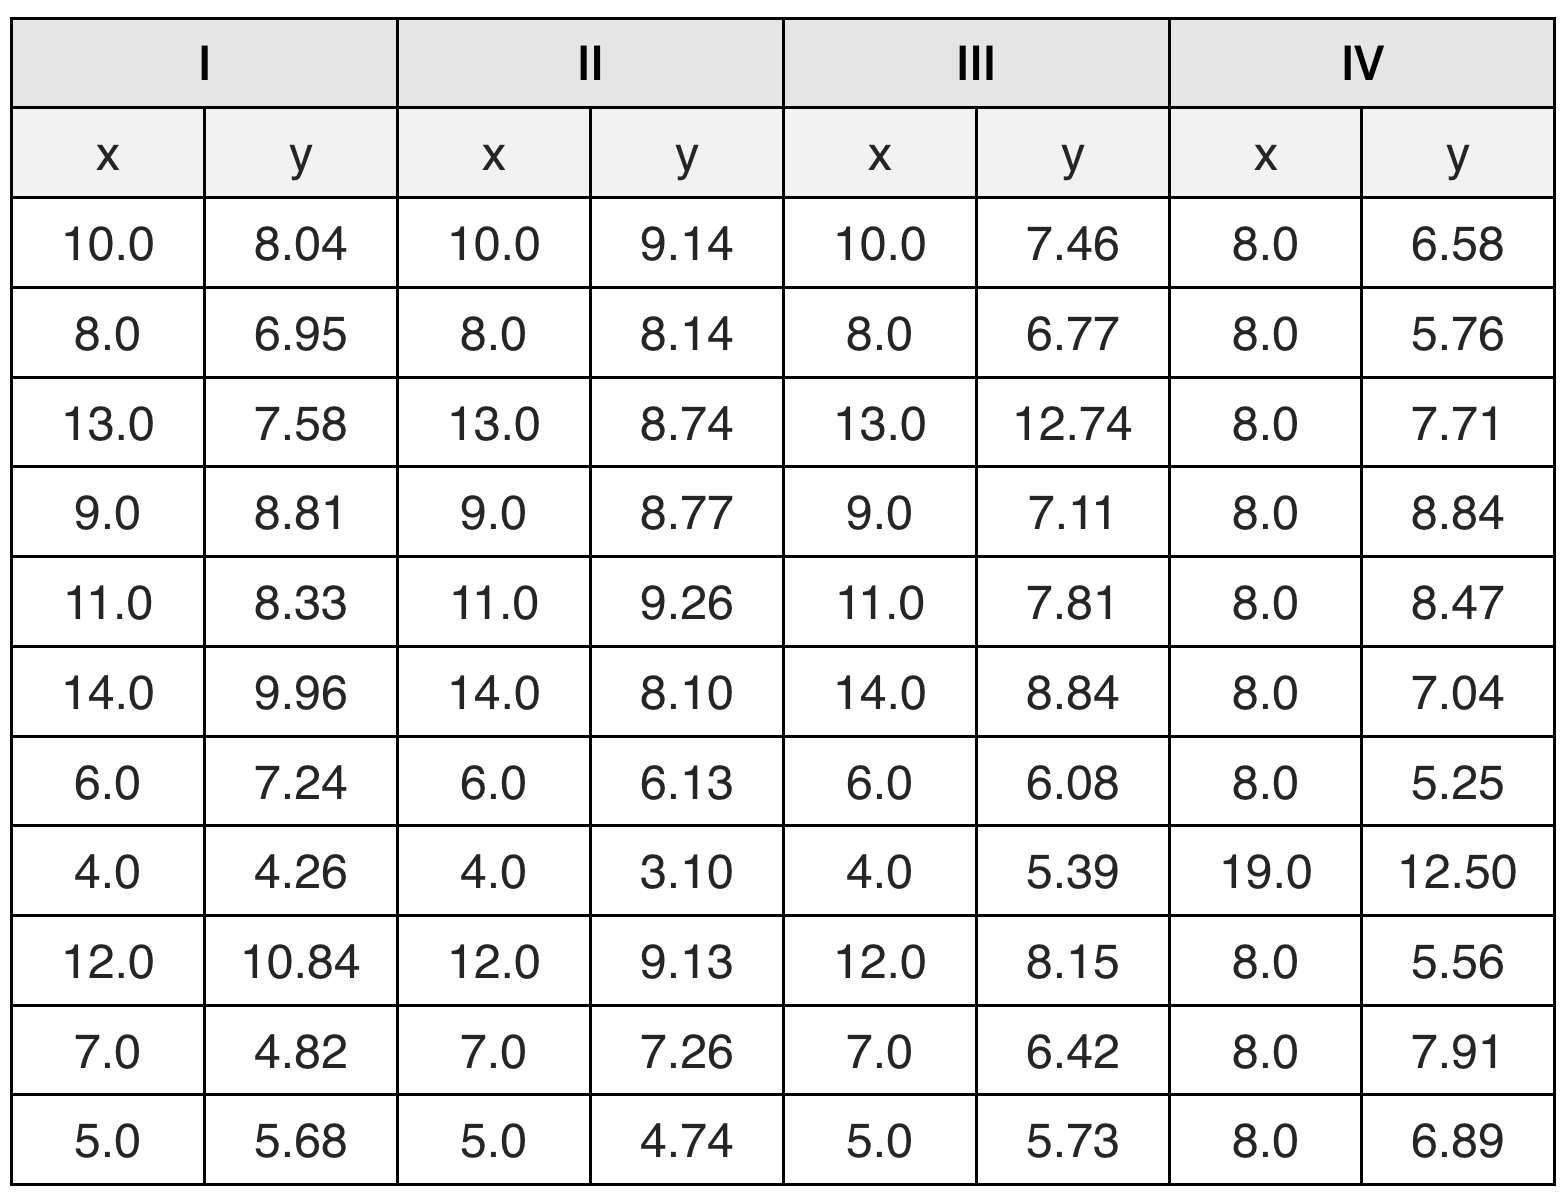
\includegraphics[width=.85\textwidth]{Anscombe-tables.png}
    \end{column}
  \end{columns}
%  \vfill
%  Data at \url{http://www.labri.fr/perso/nrougier/tmp/Anscombe.csv}\\

\end{frame}


% -----------------------------------------------------------------------------
\begin{frame}{Anscombe's Quartet}
  \begin{columns}
    \begin{column}{.5\textwidth}    
      What is common to these data sets?\\
      ~\\
      \begin{tabular}{ll}
        Mean of x            & 9\\
        Sample variance of x & 11\\
        Mean of y            & 7.5\\
        Sample variance of y & 4.12\\
        Linear regression    & y=3.00+0.500*x\\
        R squared            & 0.666\\
        p value              & 0.0021\\
      \end{tabular}

    \end{column}
    \begin{column}{.5\textwidth}
      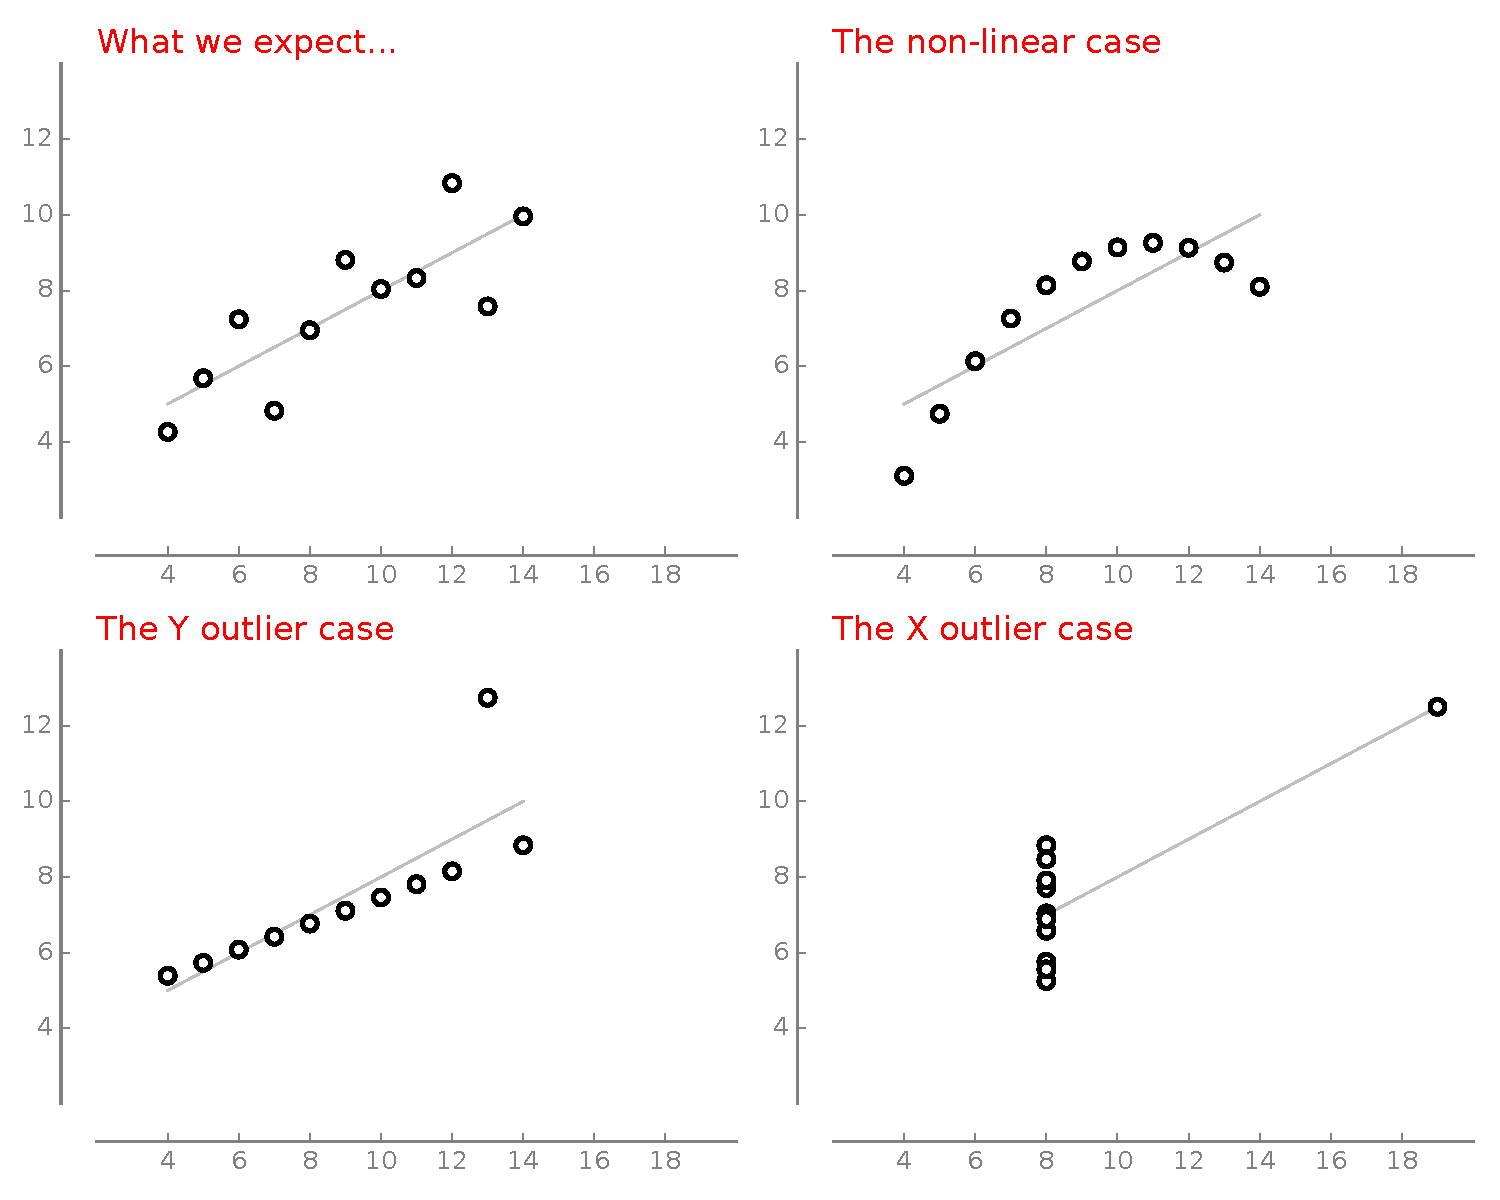
\includegraphics[width=\textwidth]{Anscombe-plots.pdf}
    \end{column}
  \end{columns}

\vfill
\noindent A computer should make both calculations and graphs -- {\em Francis Anscombe (1918-2001)}
  
\end{frame}

%% % -----------------------------------------------------------------------------
%% \begin{frame}{Anscombe's Quartet}
%%   \begin{quote}
%%     {\Large A computer should make both calculations and graphs.}
%%     \begin{flushright}
%%       \em \small Francis Anscombe (1918-2001)
%%     \end{flushright}
%%   \end{quote}
%%   \vfill
%%   \begin{quote}
%%     {\Large The purpose of computing is insight, not numbers.}
%%     \begin{flushright}
%%       \em \small Richard Hamming, 1962
%%     \end{flushright}
%%   \end{quote}
%% \end{frame}



% -----------------------------------------------------------------------------
\begin{frame}{Cholera epidemic, London, 1854}
  \begin{columns}
    \begin{column}{.3\textwidth}
      John Snow (1813-1858) is considered one of the fathers of modern
      epidemiology, in part because of his work in tracing the source of a
      cholera outbreak in Soho, London, in 1854.
    \end{column}
    \begin{column}{.6\textwidth}
      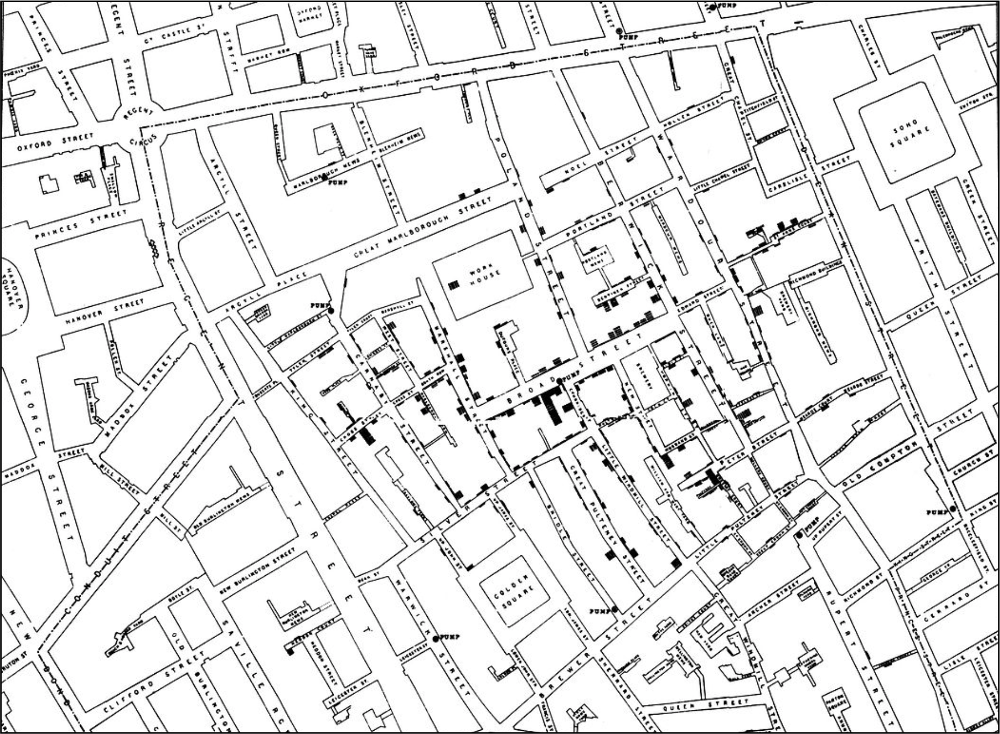
\includegraphics[width=\textwidth]{cholera-old.png}
    \end{column}
  \end{columns}
\end{frame}

% -----------------------------------------------------------------------------
\begin{frame}{Cholera epidemic, London, 1854}
  \begin{columns}
    \begin{column}{.3\textwidth}
      John Snow (1813-1858) is considered one of the fathers of modern
      epidemiology, in part because of his work in tracing the source of a
      cholera outbreak in Soho, London, in 1854.
    \end{column}
    \begin{column}{.6\textwidth}
      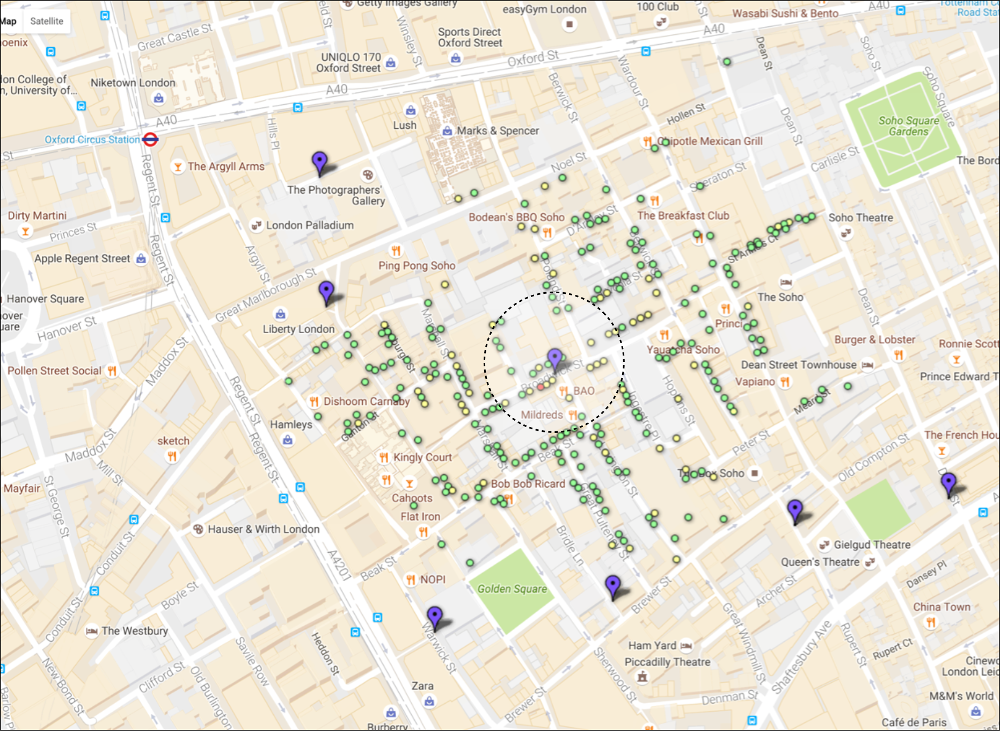
\includegraphics[width=\textwidth]{cholera-modern.png}
    \end{column}
  \end{columns}
\end{frame}

% -----------------------------------------------------------------------------
\begin{frame}{What is data visualisation?}
  \begin{quote}
    Visualisation is a method of computing. It transforms the symbolic into the
    geometric, enabling researchers to observe their simulations and
    computations. Visualisation offers a method for seeing the unseen. It
    enriches the process of scientific discovery and fosters profound and
    unexpected insights.
    \begin{flushright}
      \em \small Visualisation in Scientific Computing, NSF report, 1987
    \end{flushright}
  \end{quote}
\end{frame}

% -----------------------------------------------------------------------------
\begin{frame}{The Visualization pipeline}
  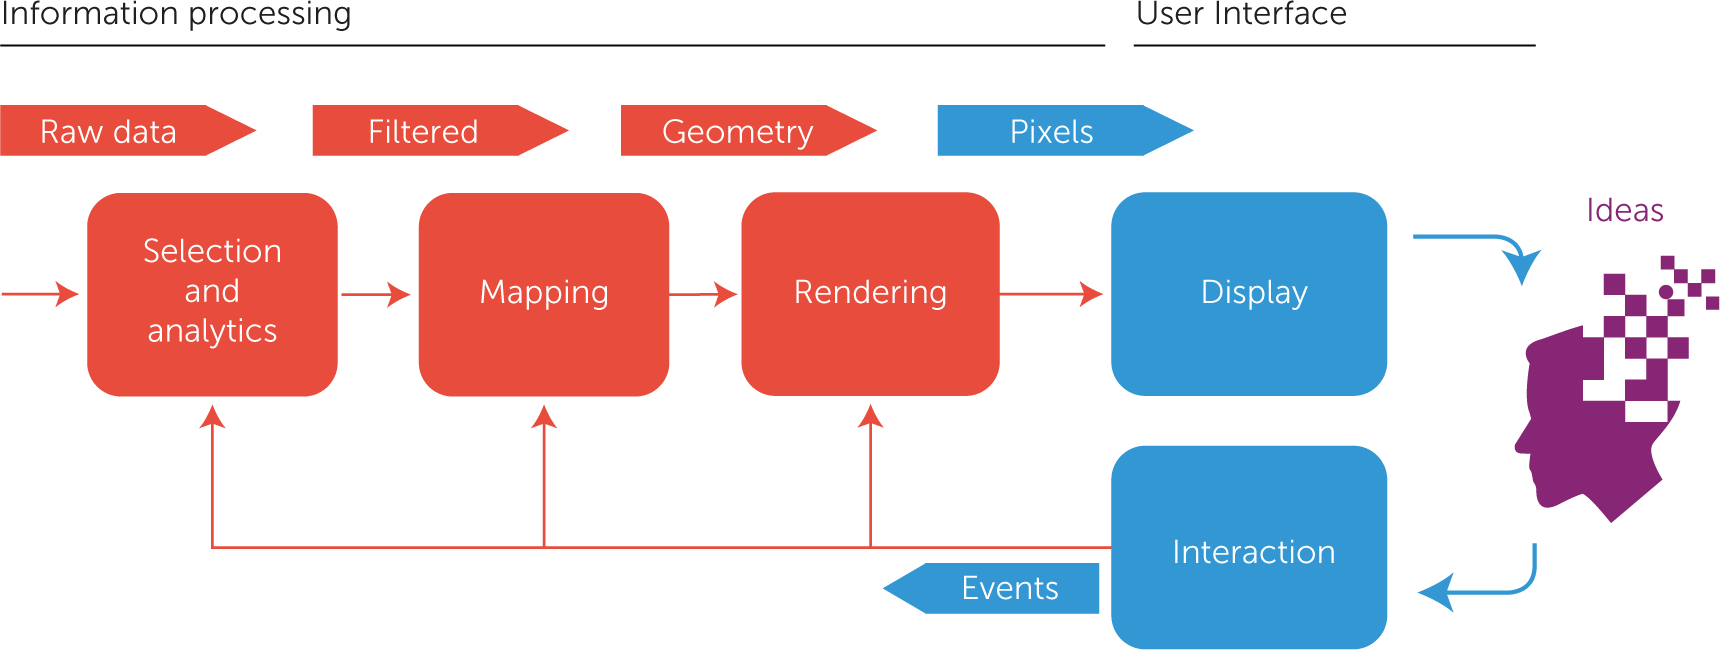
\includegraphics[width=\textwidth]{pipeline.png}
  ~\\
  From Scalable Real-Time Visualization Using the Cloud,
  Holliman \& Watson, 2015.\\
\end{frame}


% -----------------------------------------------------------------------------
\begin{frame}{Quantitative vs Qualitative data}

  \textbf{Quantitative}
         (values or observations that can be measured)\\
  \begin{itemize}
  \item Continuous (e.g. temperature) 
  \item Discrete (e.g. number of inhabitants)
  \end{itemize}
  \vfill
  \textbf{Qualitative}
         (values or observations that can be sorted into groups or categories)\\
  \begin{itemize}
  \item Nominal (e.g. nationality)
  \item Ordinal (e.g. months)
  \item Interval (e.g. age groups)
  \end{itemize}
  
\end{frame}

% -----------------------------------------------------------------------------
\begin{frame}{Graphical elements}
  A scientific figure can be fully described by a set of graphic primitives
  with different attributes:
  \begin{itemize}
  \item Points, markers, lines, areas, ...
  \item Position, color, shape, size, orientation, curvature, ...
  \item Helpers, text, axis, ticks, ...
  \item Interaction, animation, ...
  \end{itemize}
  
  Questions is thus how to organize and link them to the underlying data.
\end{frame}

% -----------------------------------------------------------------------------
\begin{frame}{Principles of visual perception}
  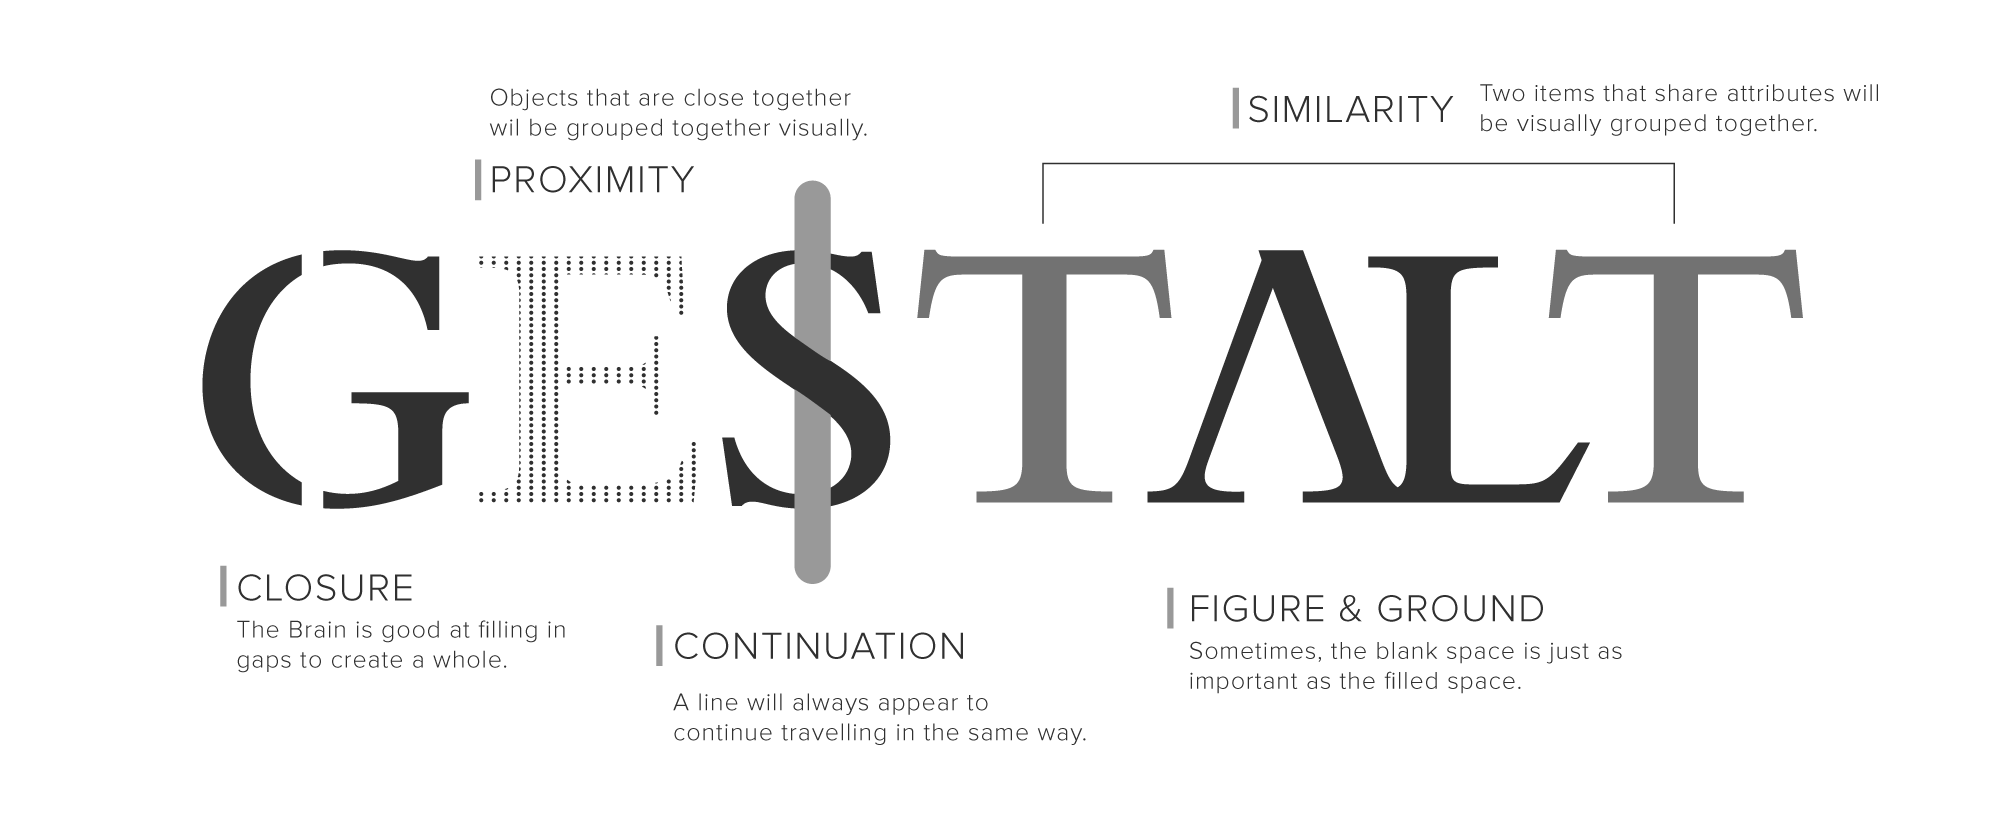
\includegraphics[width=\textwidth]{gestalt.png}
\end{frame}

% -----------------------------------------------------------------------------
\begin{frame}{Visualization Analysis and Design (T. Munzner)}
  \begin{center}
    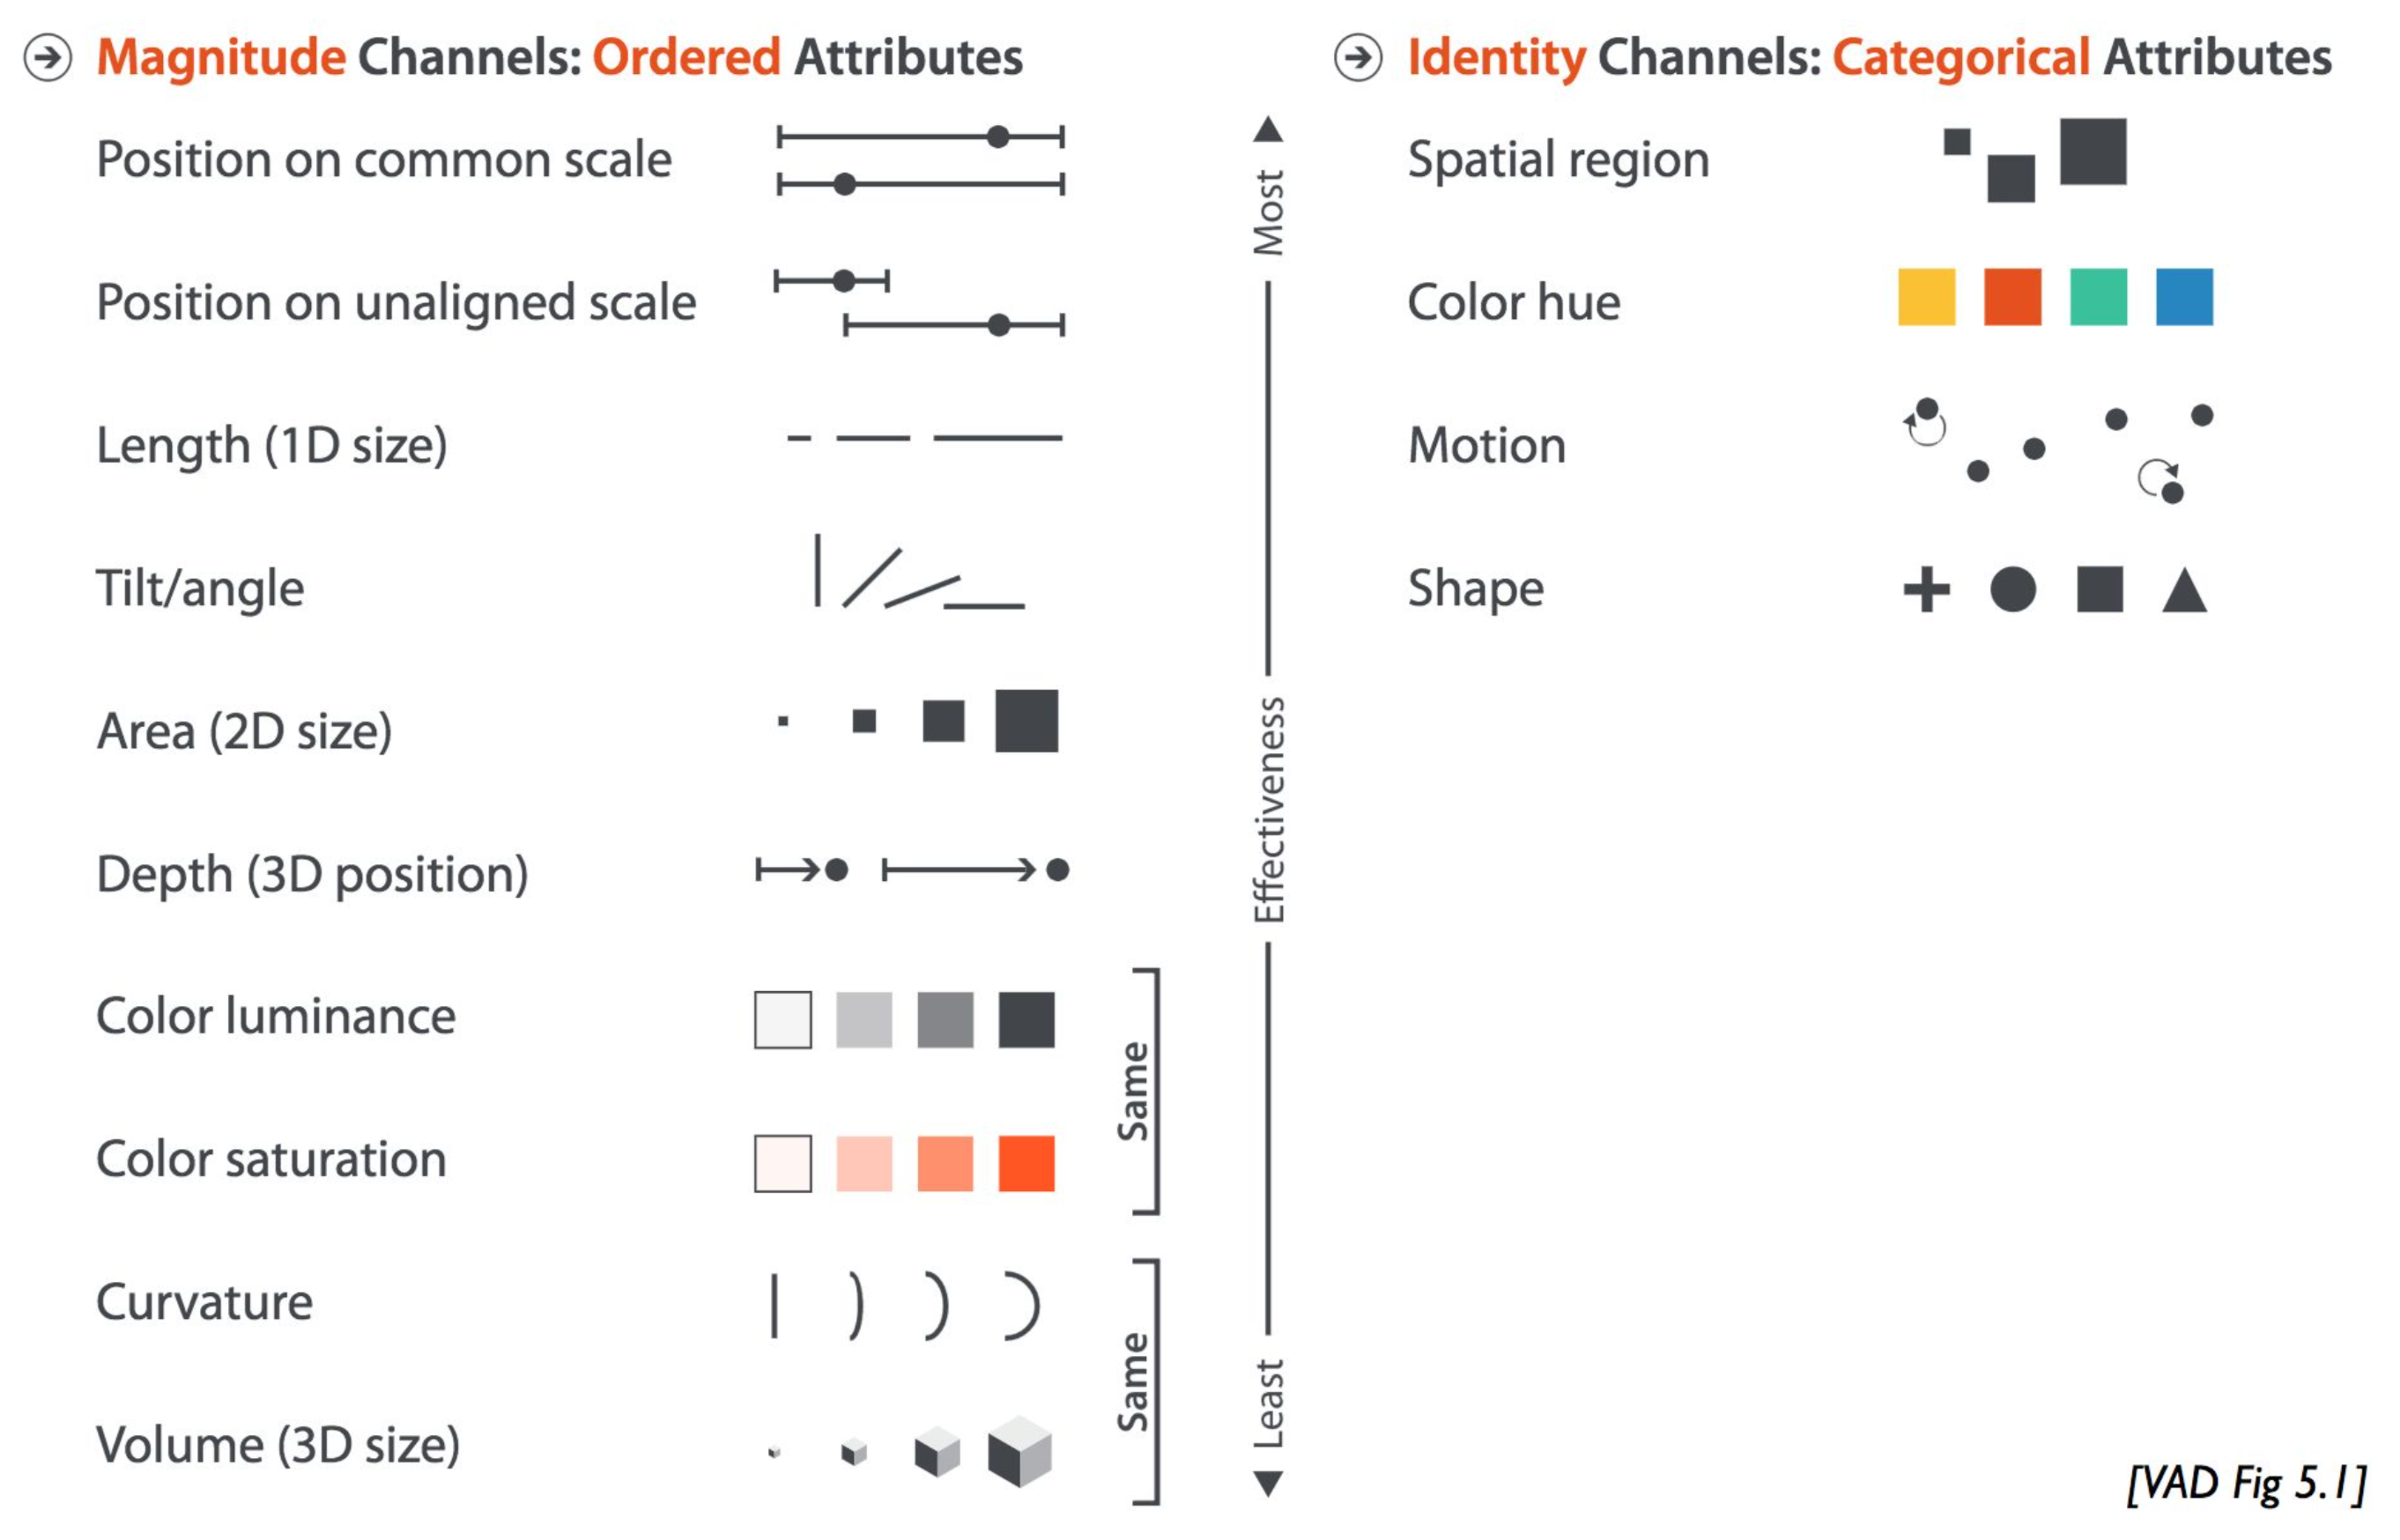
\includegraphics[width=.75\textwidth]{VAD.png}
  \end{center}
\end{frame}

% -----------------------------------------------------------------------------
\begin{frame}{Data Visualization catalogue (S. Recebba)}
  \begin{center}
    \href{https://datavizcatalogue.com/}{
    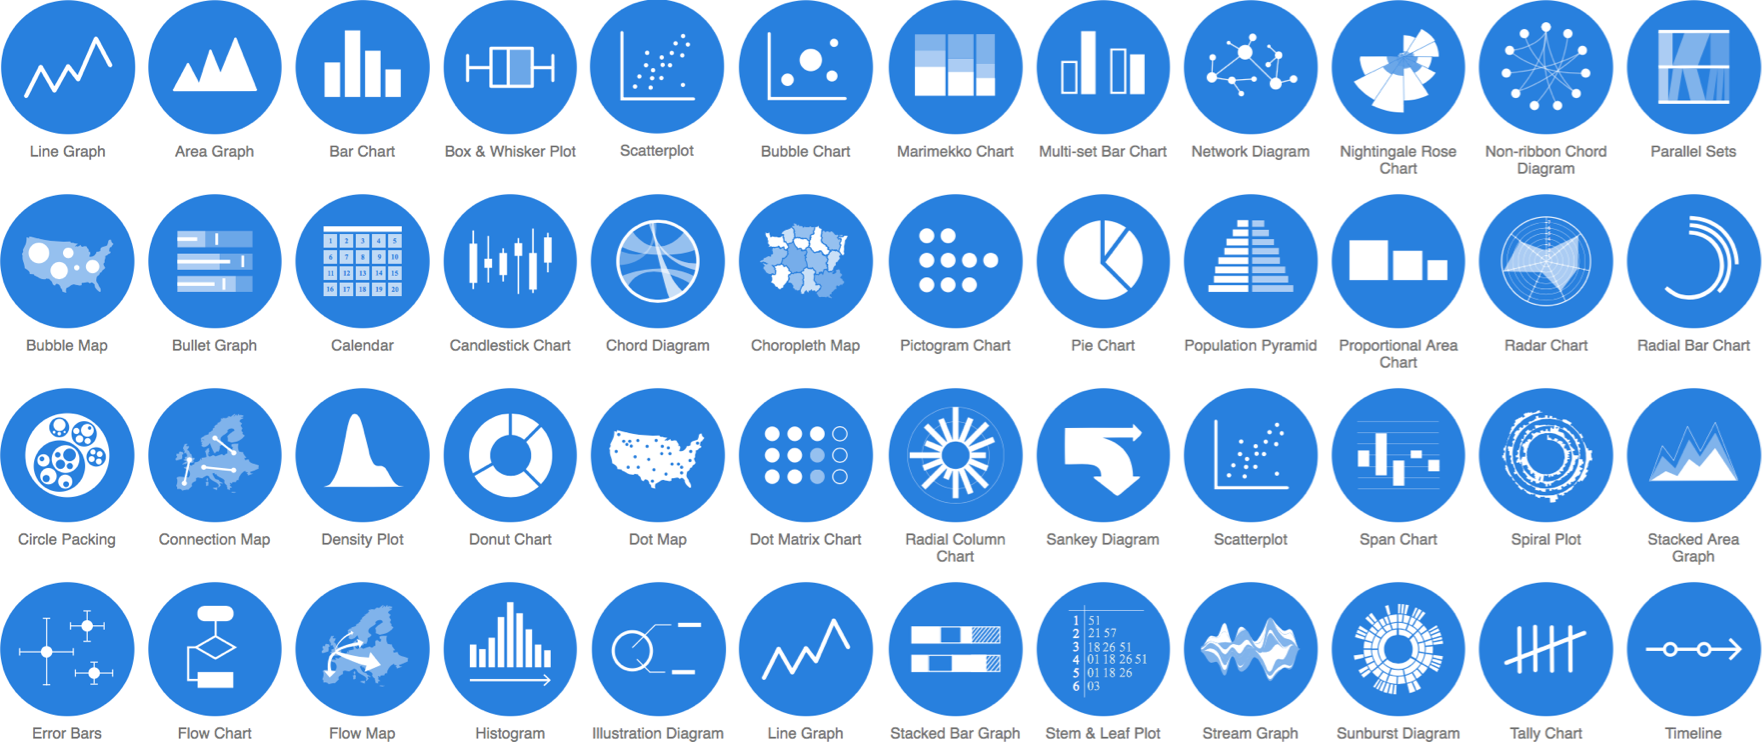
\includegraphics[width=\textwidth]{catalogue.png}}\\
  \end{center}
  {\tt datavizcatalogue.com}
\end{frame}


% -----------------------------------------------------------------------------
%% \begin{frame}{Chart Suggestions - A Thought-Starter (A. Abela)}
%%   \begin{center}
%%     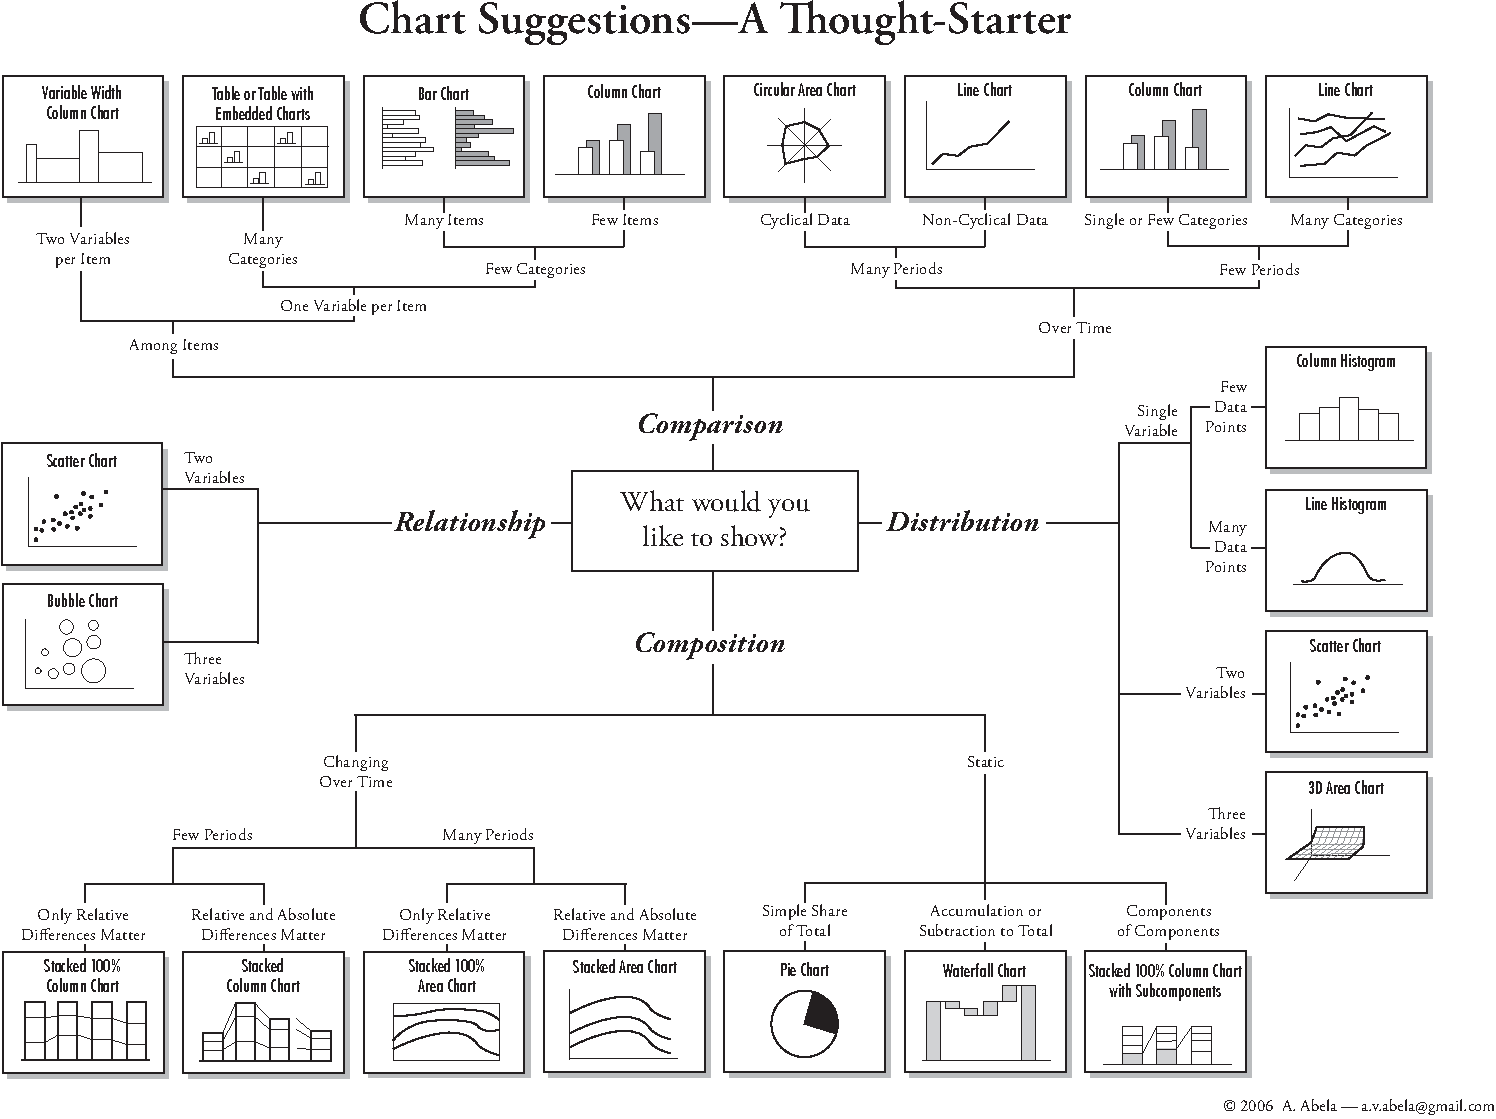
\includegraphics[width=.75\textwidth]{chart.pdf}
%%   \end{center}
%% \end{frame}


  
% =============================================================================
\section{Ten~simple~rules~for~better~figures}
% =============================================================================

% -----------------------------------------------------------------------------
\begin{frame}{Rule 1: Know your audience}
  \begin{center}
    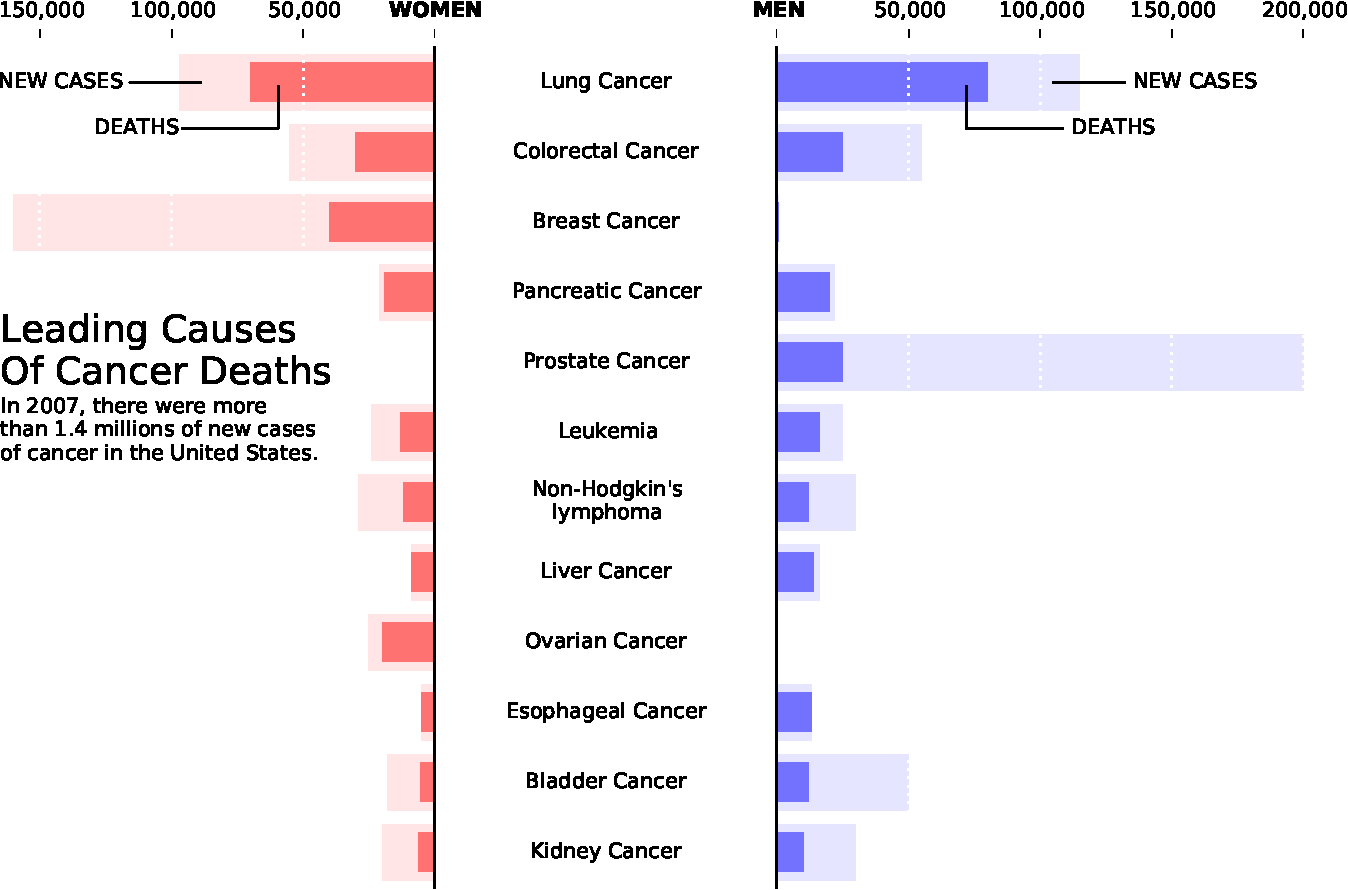
\includegraphics[width=.75\textwidth]{rule-1.pdf}
  \end{center} 
\end{frame}

% -----------------------------------------------------------------------------
\begin{frame}{Rule 2: Identify your message}
  \begin{center}
    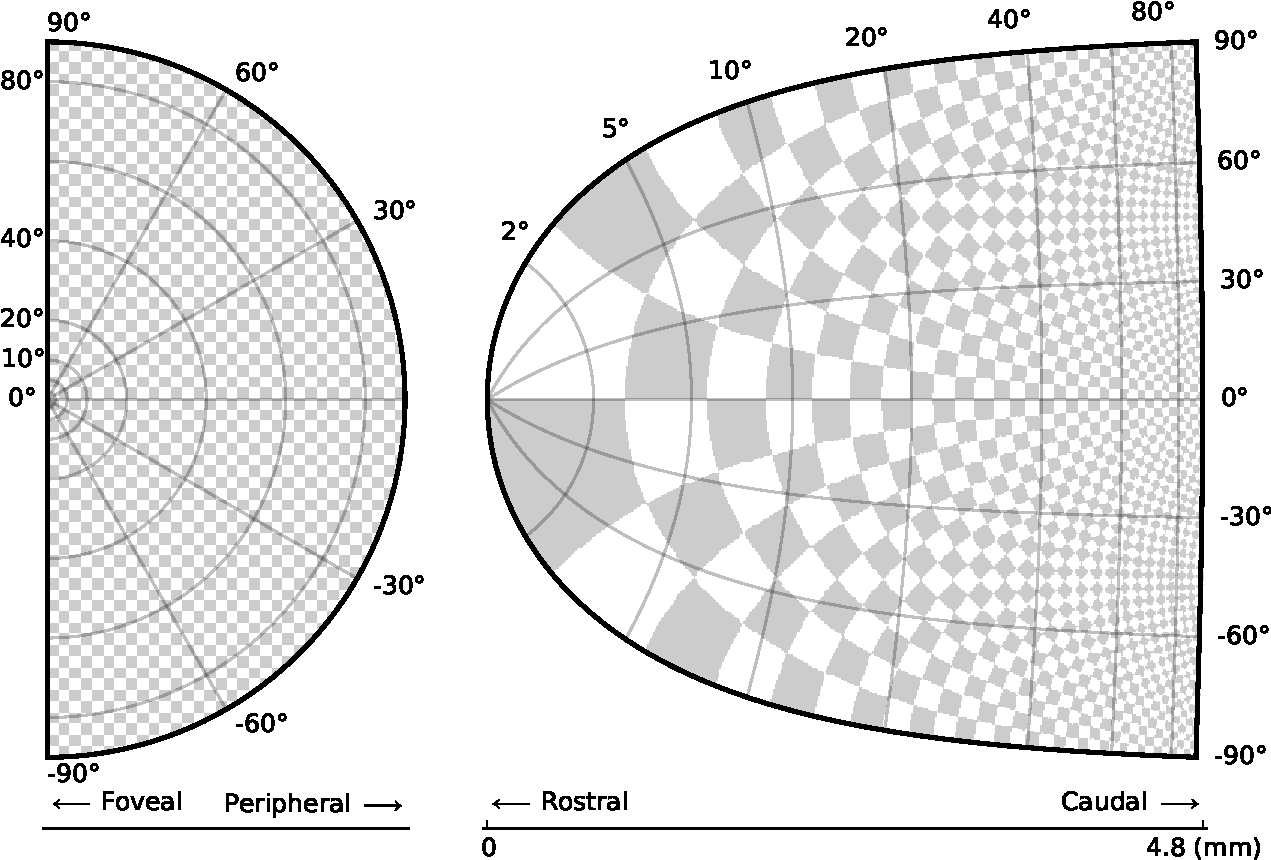
\includegraphics[width=.75\textwidth]{rule-2.pdf}
  \end{center} 
\end{frame}

% -----------------------------------------------------------------------------
\begin{frame}{Rule 3: Adapt the figure}
  \begin{center}
    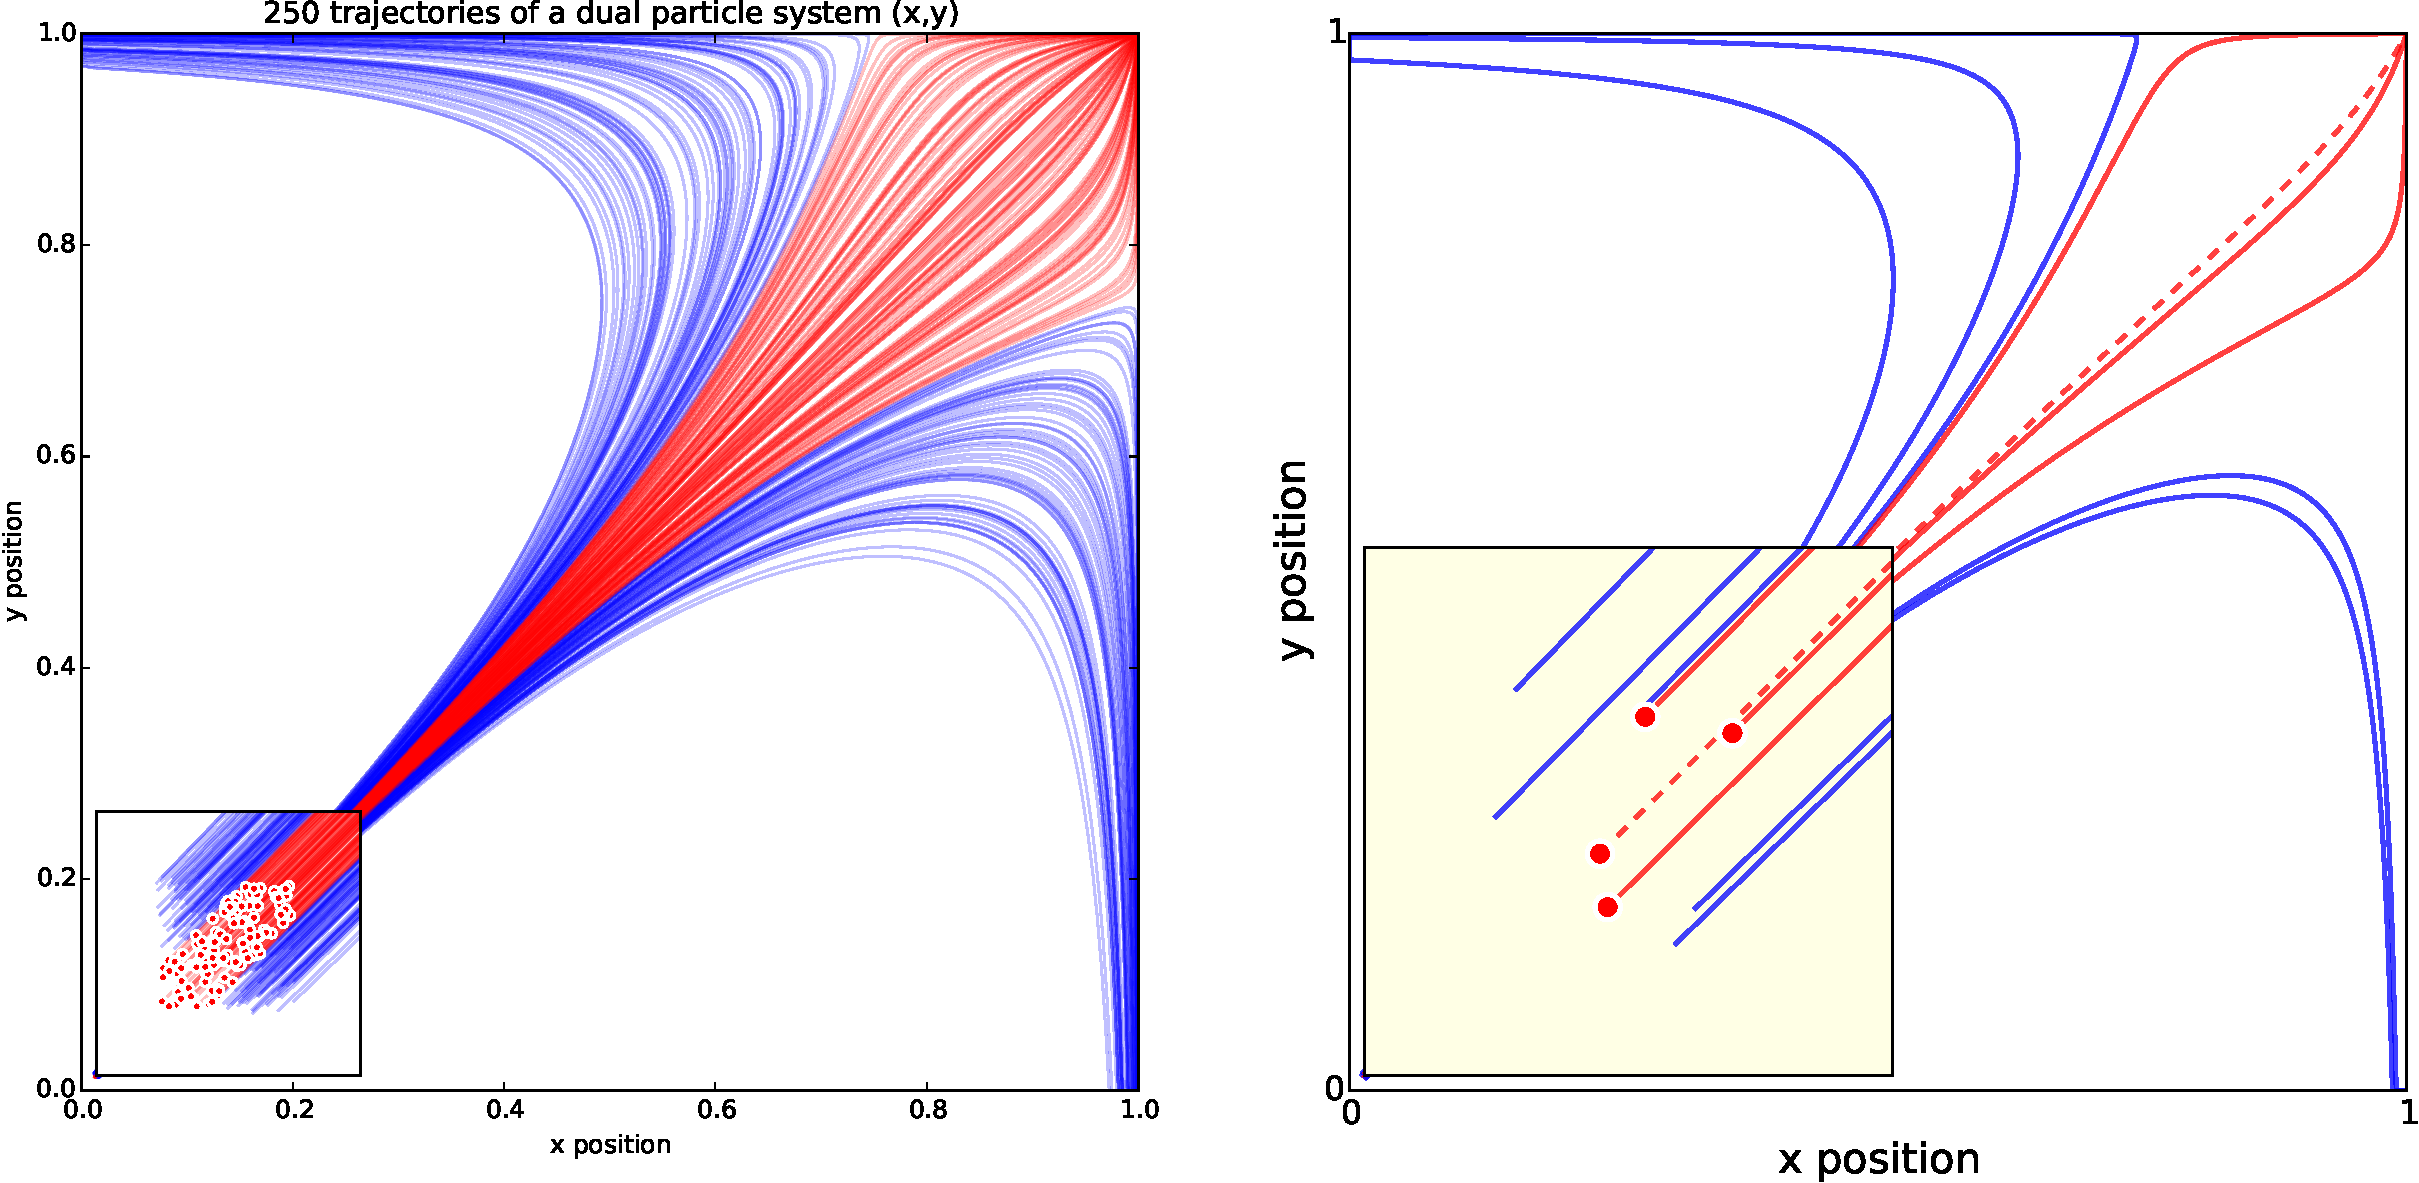
\includegraphics[width=\textwidth]{rule-3.pdf}
  \end{center} 
\end{frame}

% -----------------------------------------------------------------------------
\begin{frame}{Rule 4: Captions are not optional}

  \begin{columns}
    \begin{column}{.45\textwidth}
        \begin{center}
          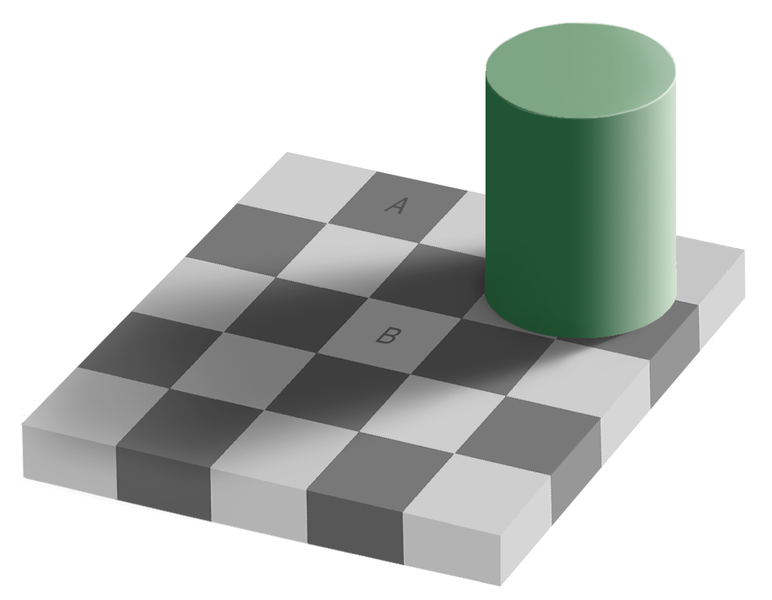
\includegraphics[width=.95\textwidth]{rule-4.png}
        \end{center}
    \end{column}
    \begin{column}{.45\textwidth}
        \begin{center}
          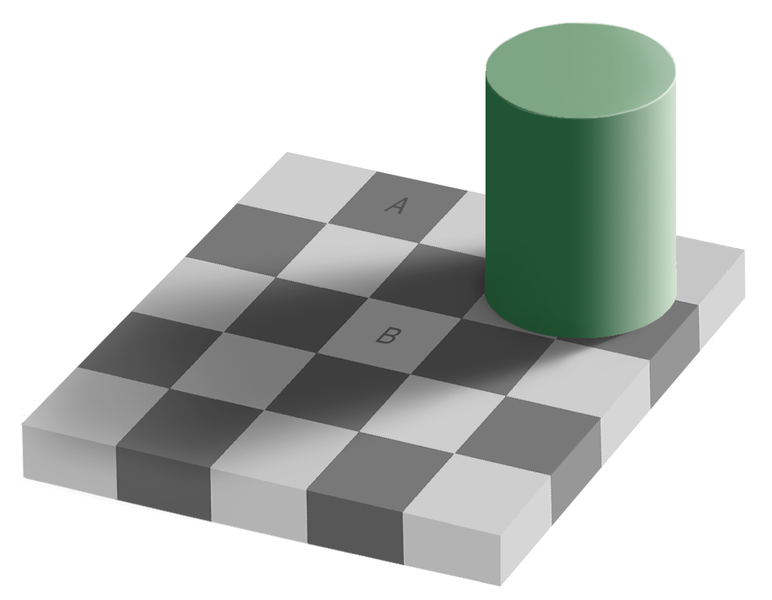
\includegraphics[width=.95\textwidth]{rule-4.png}
        \end{center}
    \end{column}
  \end{columns}
  \begin{columns}
    \begin{column}{.45\textwidth}
        \begin{center}
          Optical illusion
        \end{center}
    \end{column}
    \begin{column}{.45\textwidth}
        \begin{center}
          The A and B patches are actually the same color even
          though we perceived them at being different color.
        \end{center}
    \end{column}
  \end{columns}


\end{frame}

% -----------------------------------------------------------------------------
\begin{frame}{Rule 5: Do not trust the defaults}
  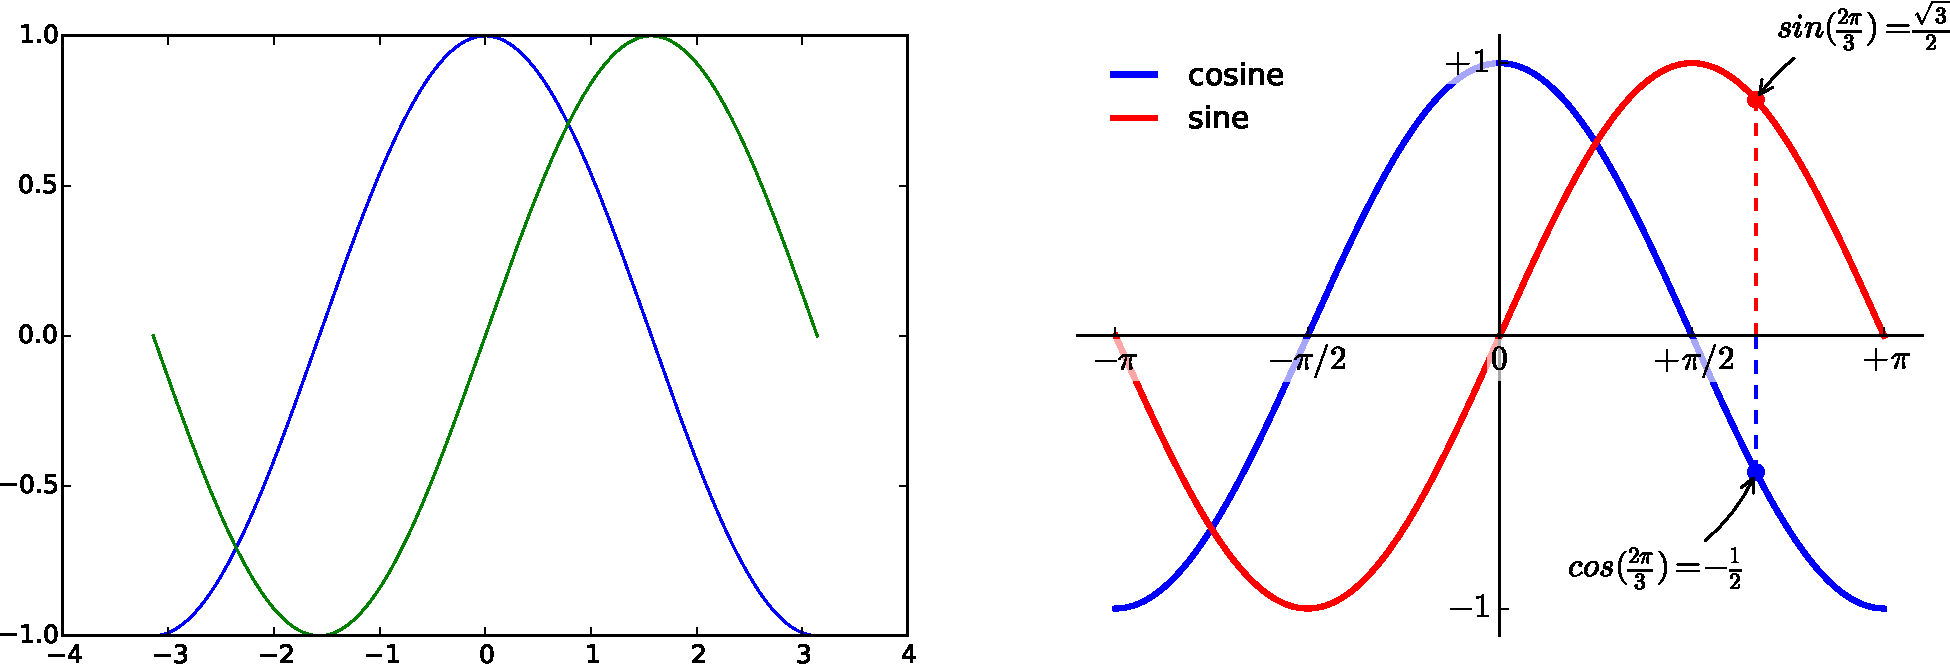
\includegraphics[width=\textwidth]{rule-5.pdf}
\end{frame}

% -----------------------------------------------------------------------------
\begin{frame}{Rule 6: Use color effectively}
  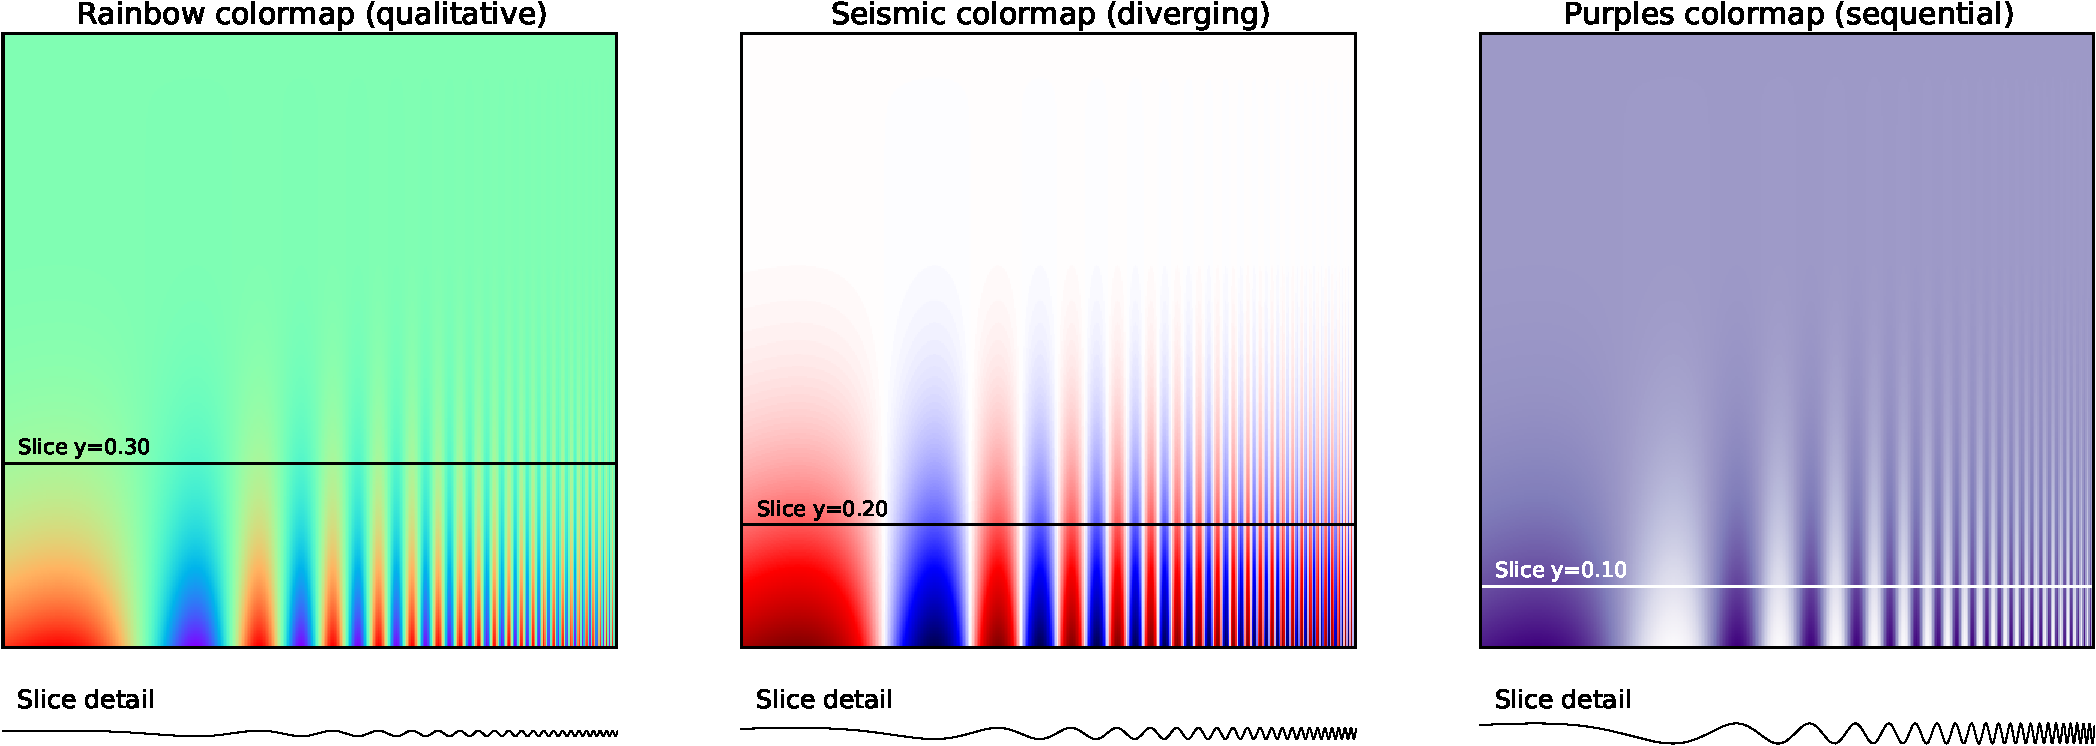
\includegraphics[width=\textwidth]{rule-6.pdf}
\end{frame}

% -----------------------------------------------------------------------------
\begin{frame}{Rule 6 bis: Above all, no jet. Ever.}
  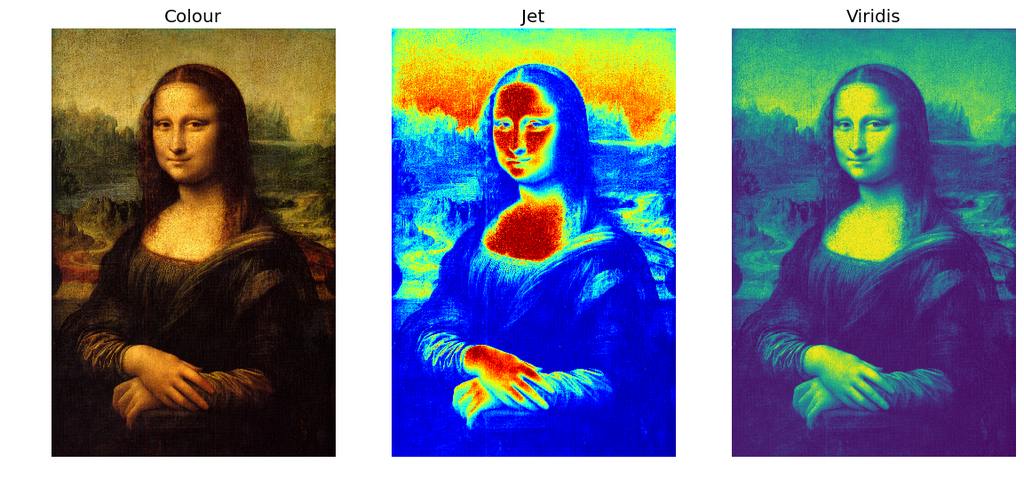
\includegraphics[width=\textwidth]{rule-6bis.png}
\end{frame}

% -----------------------------------------------------------------------------
\begin{frame}{Rule 7: Do not mislead the reader}
  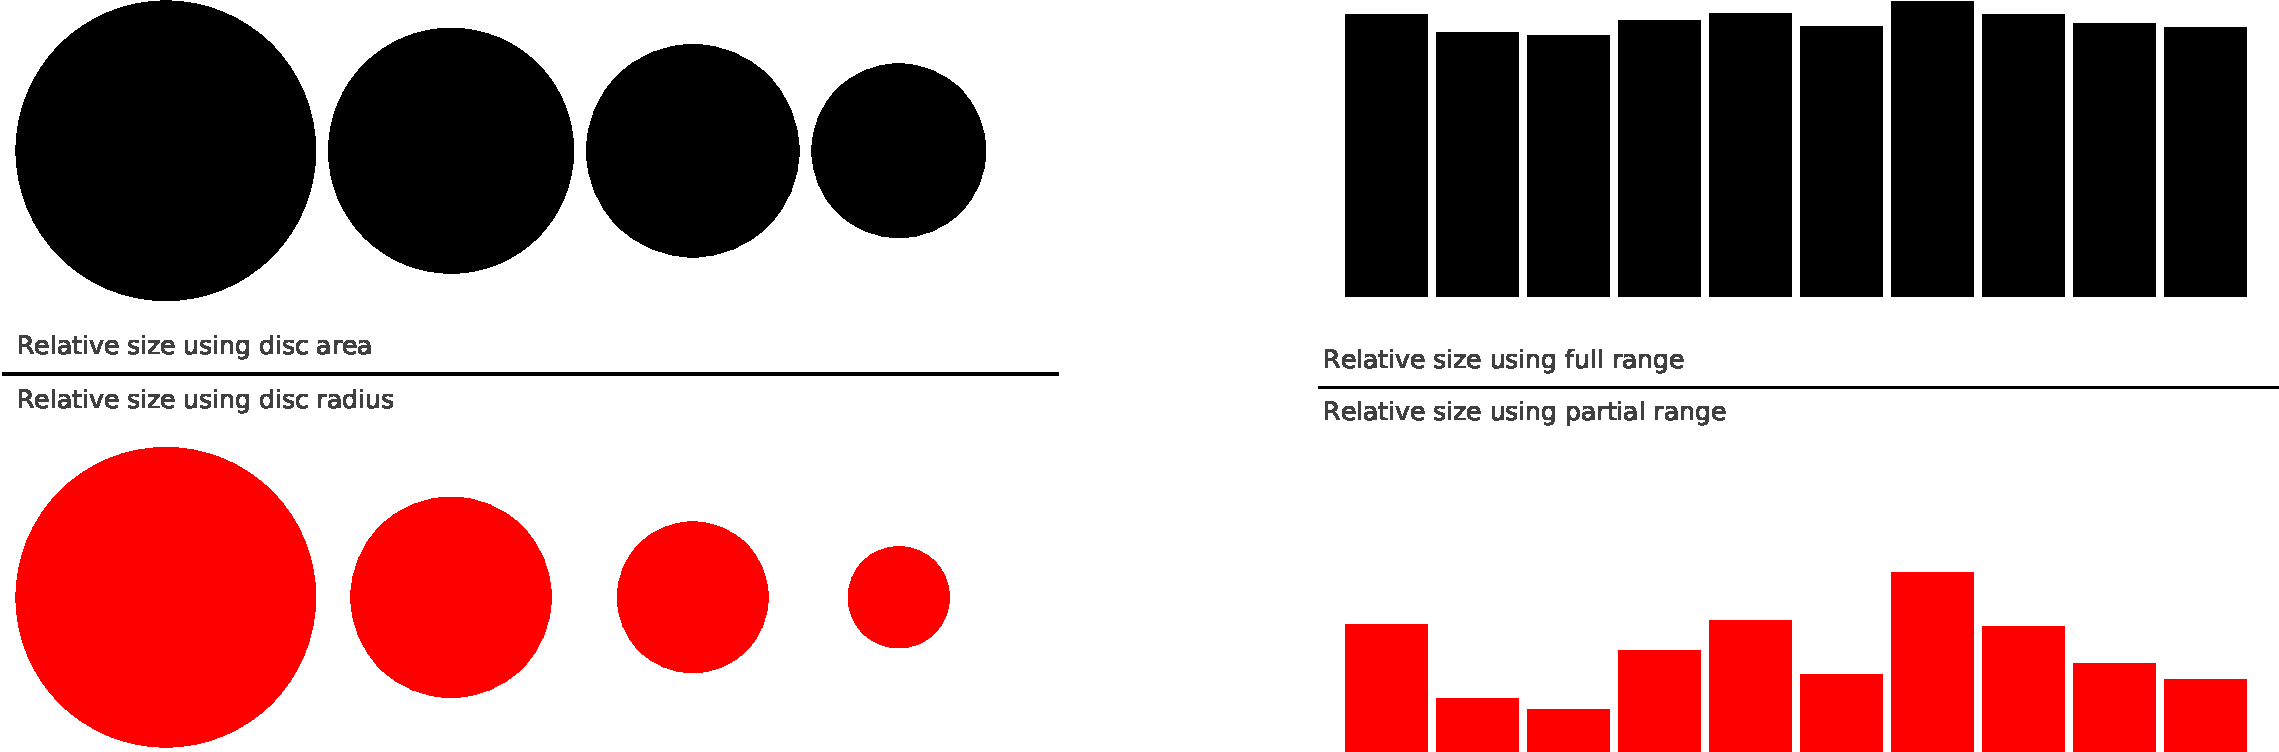
\includegraphics[width=\textwidth]{rule-7.pdf}
\end{frame}

\begin{frame}{Rule 7: Do not mislead the reader. Really.}
  \begin{center}
    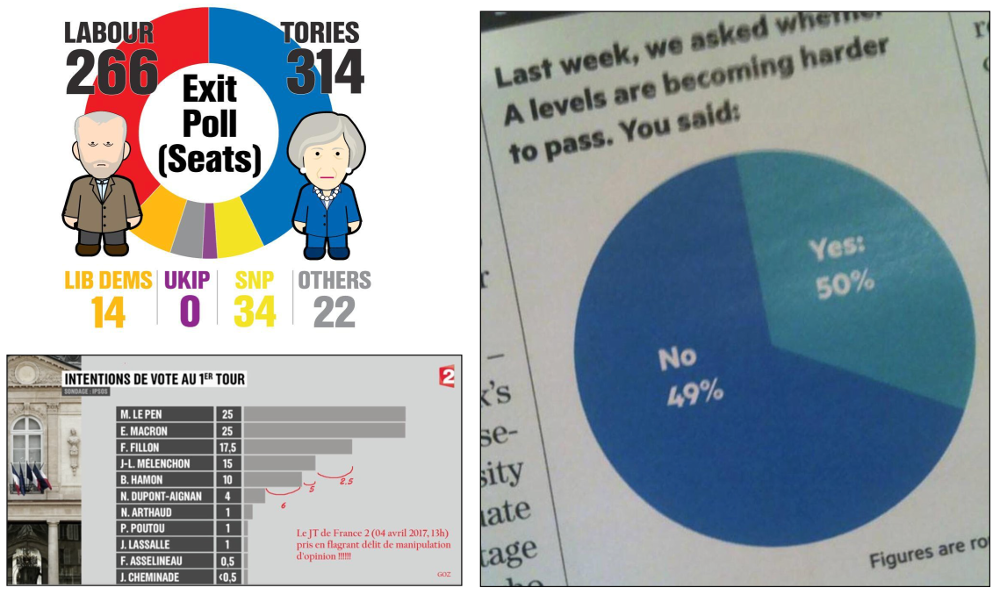
\includegraphics[width=.75\textwidth]{rule-7bis.png}
  \end{center}
\end{frame}

% -----------------------------------------------------------------------------
\begin{frame}{Rule 8: Avoid chartjunk}
  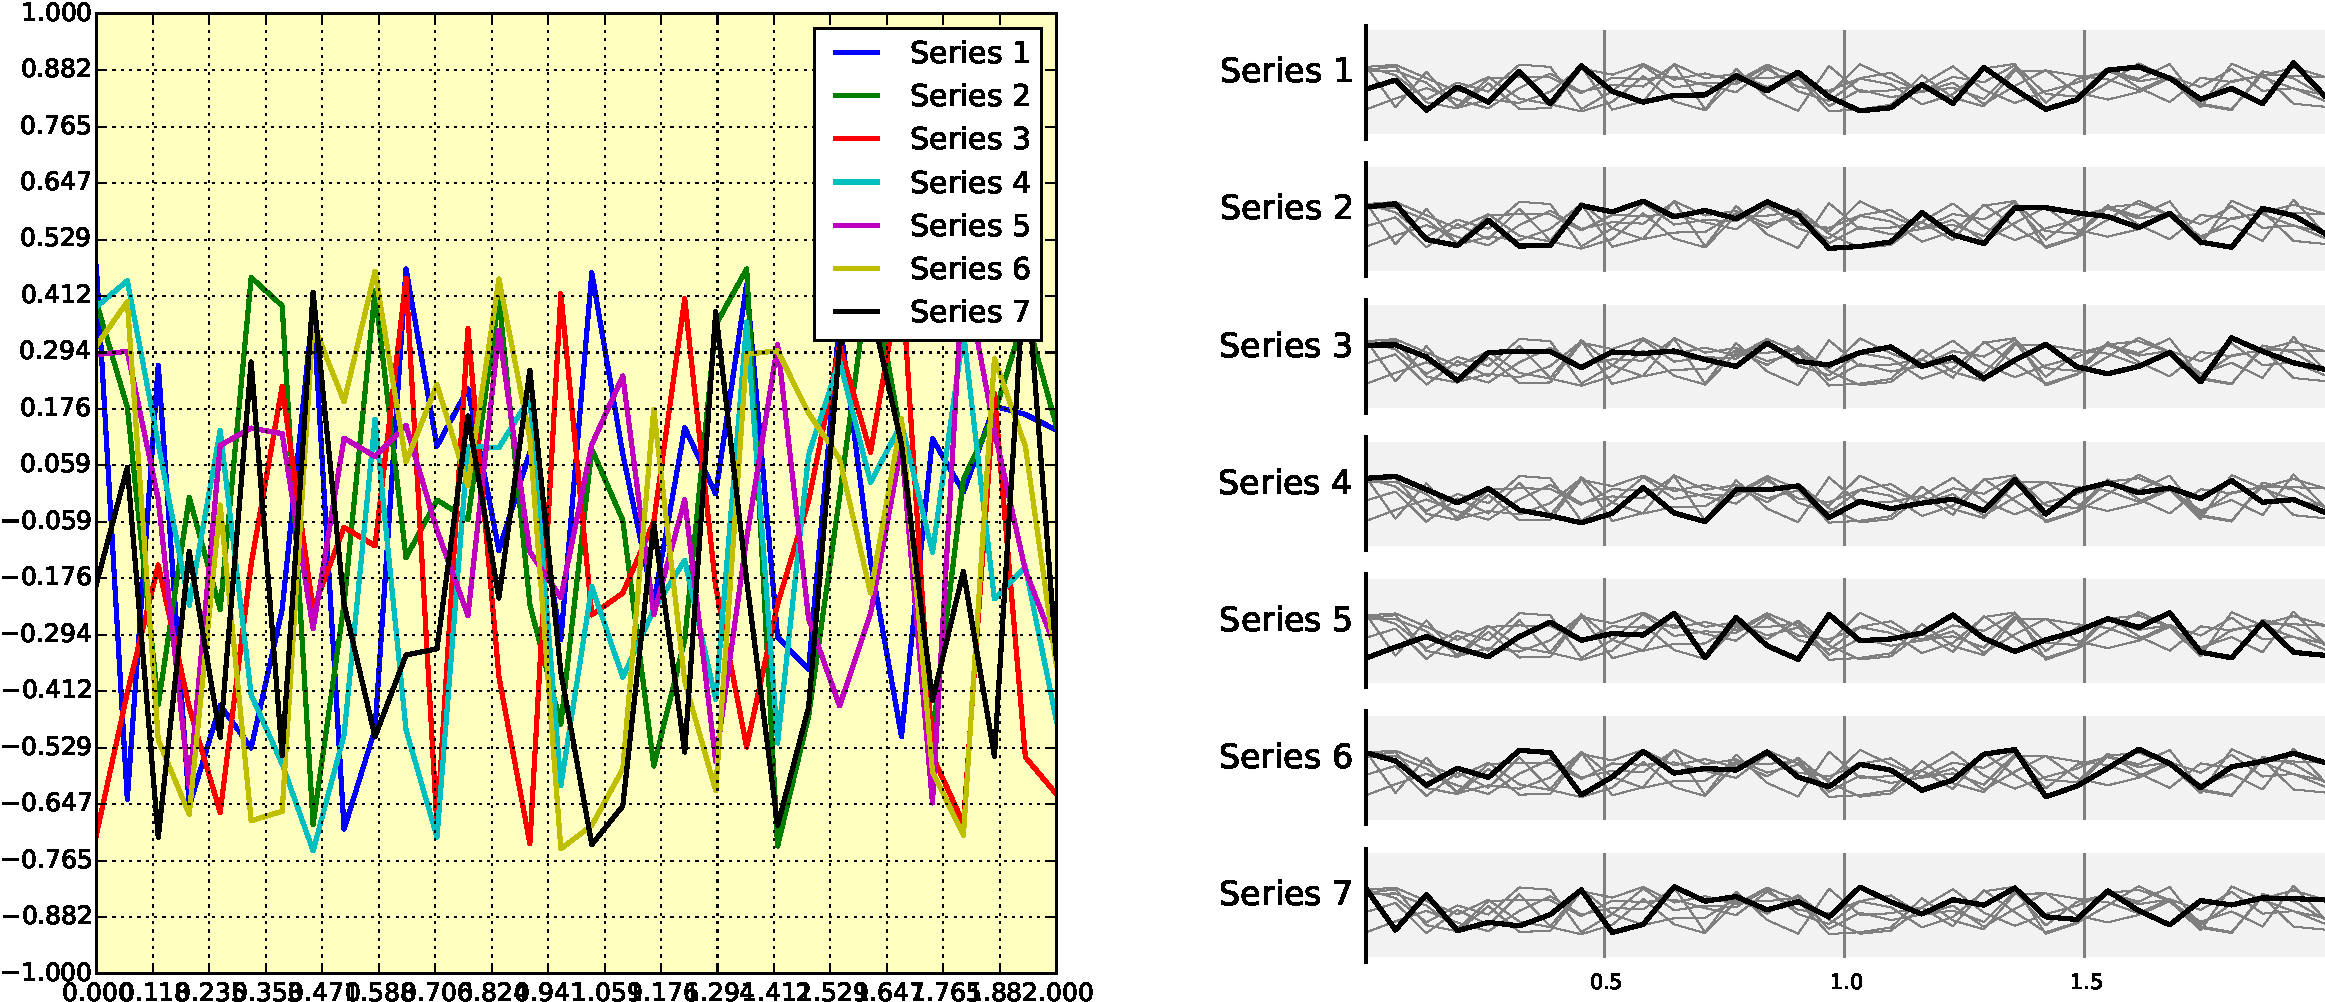
\includegraphics[width=\textwidth]{rule-8.pdf}
\end{frame}

% -----------------------------------------------------------------------------
\begin{frame}{Rule 8 bis: Less is more}
  \begin{center}
    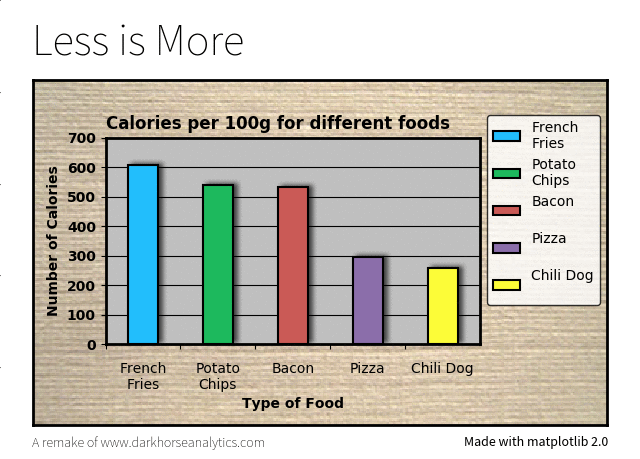
\includegraphics[width=.75\textwidth]{rule-8bis.png}
  \end{center}
\end{frame}

% -----------------------------------------------------------------------------
\begin{frame}{Rule 9: Message trumps beauty}
  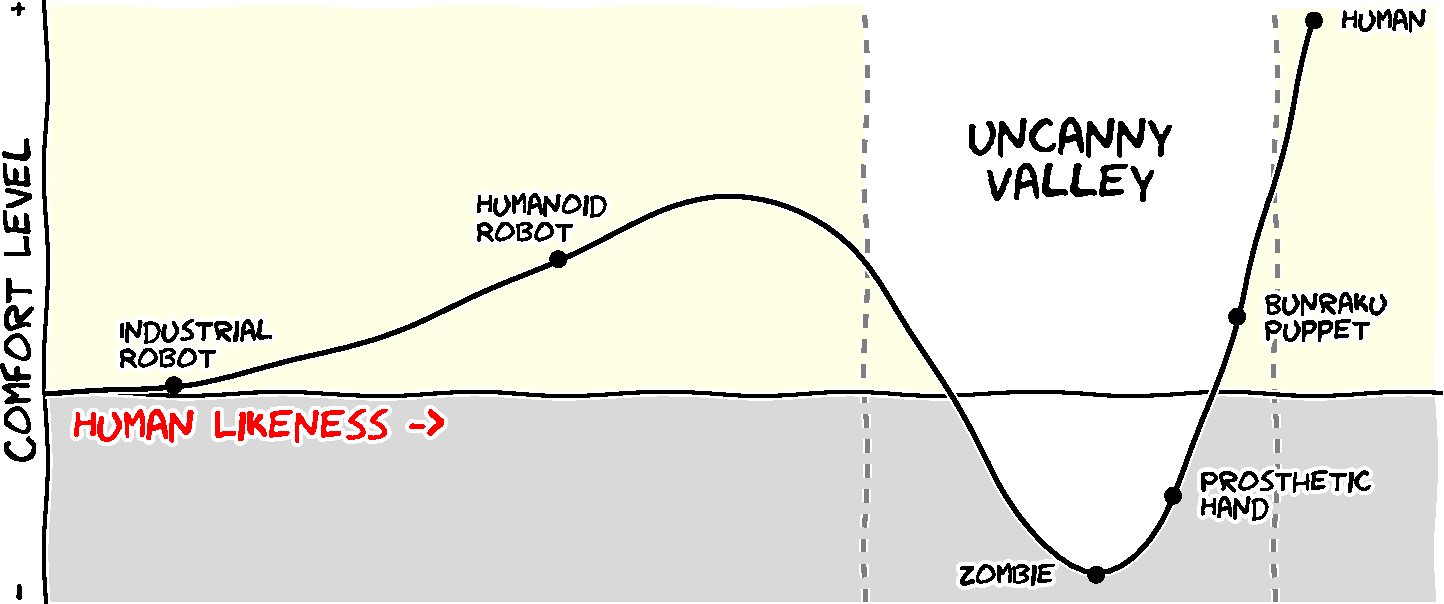
\includegraphics[width=\textwidth]{rule-9.pdf}
\end{frame}

% -----------------------------------------------------------------------------
\begin{frame}{Rule 10: Get the right tool}
  \begin{itemize}
  \item PDFCrop (remove white borders)\\
    \url{http://pdfcrop.sourceforge.net}
  \item GraphViz (easy graph)\\
    \url{http://www.graphviz.org}
  \item ImageMagick (scripted image processing)\\
    \url{http://www.imagemagick.org/script/index.php}
  \item Gimp (bitmap image manipulation)\\
    \url{https://www.gimp.org}
  \item Inkscape (vector image manipulation)\\
    \url{https://www.inkscape.org}
  \item Tikz (scripted vector art)\\
    \url{http://www.texample.net/tikz/examples/all/}
  \item And many, many, many others …
  \end{itemize}
\end{frame}

% -----------------------------------------------------------------------------
\begin{frame}{Rule 10: Get the right tool}
    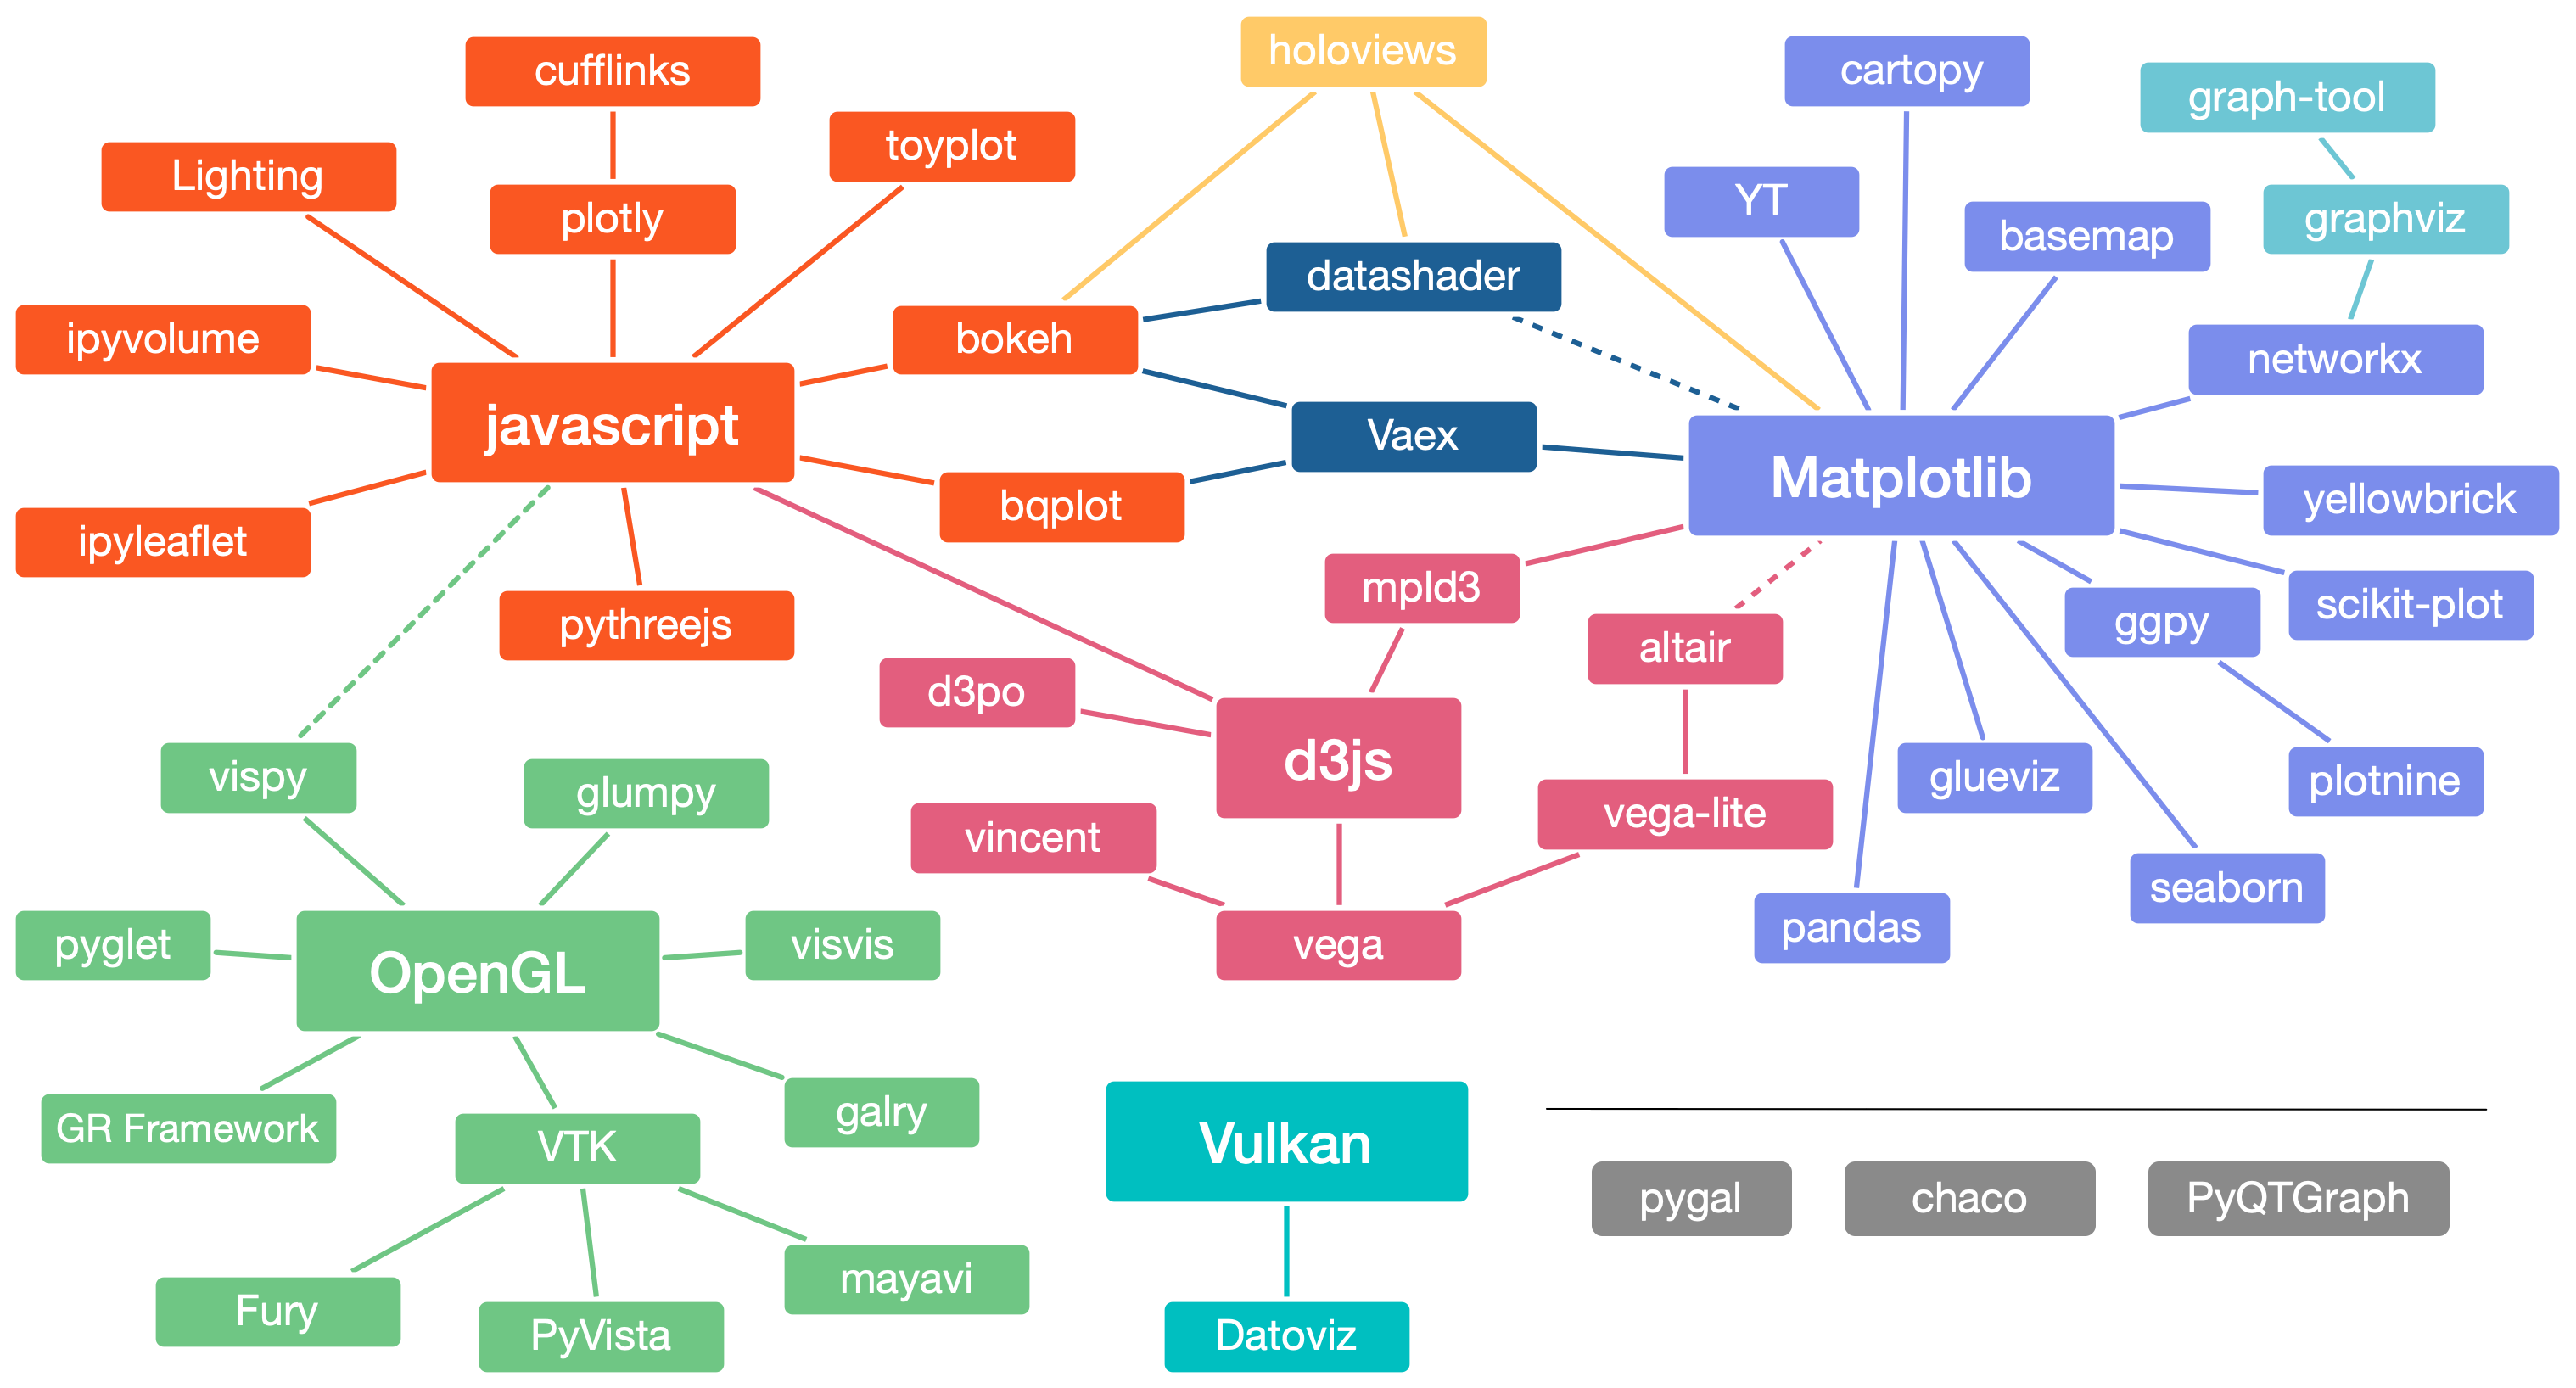
\includegraphics[width=\textwidth]{rule-10bis.png}
\end{frame}


% -----------------------------------------------------------------------------
%% \begin{frame}{A note about formats}
%%   \begin{block}{Standard data formats}
%%     \vspace{0pt}
%%     \begin{itemize}
%%     \item[] \textbf{CSV} -- Comma-Separated Values
%%     \item[] \textbf{JSON} -- JavaScript Object Notation
%%     \end{itemize}
%%   \end{block}
  
%%   \begin{block}{Standard vector formats}
%%     \vspace{0pt}
%%     \begin{itemize}
%%     \item[] \textbf{PDF} -- Portable Document Format
%%     \item[] \textbf{SVG} -- Scalable Vector Graphics
%%     \end{itemize}
%%   \end{block}
  
%%   \begin{block}{Standard bitmap formats}
%%     \vspace{0pt}
%%     \begin{itemize}
%%     \item[] \textbf{PNG} -- Portable Network Graphics (lossless)
%%     \item[] \textbf{JPG} -- Joint Photographic Experts Group (lossy)
%%     \end{itemize}
%%   \end{block}

%% \end{frame}


% -----------------------------------------------------------------------------
%% \begin{frame}{A note about really big data}

%%   \begin{columns}
%%     \begin{column}{.65\textwidth}
%%       \begin{block}{Analyzing 1.1 Billion NYC Taxi}
%%         \vspace{0pt}
%%     The New York City Taxi \& Limousine Commission has released a staggeringly
%%     detailed historical dataset covering over 1.1 billion individual taxi trips
%%     in the city from January 2009 through June 2015. Taken as a whole, the
%%     detailed trip-level data is more than just a vast list of taxi pickup and
%%     drop off coordinates: it’s a story of New York.
%%     \begin{flushright}
%%       \small \textnormal Todd W. Schneider
%%                          (\href{http://toddwschneider.com/}{\tt toddwschneider.com})
%%     \end{flushright}
%%       \end{block}
%%     \end{column}
%%     \begin{column}{.25\textwidth}
%%       \begin{center}
%%         \includegraphics[width=\textwidth]{./taxi_pickups_map.png}
%%       \end{center}
%%     \end{column}
%%   \end{columns}

%%   % See \url{github.com/astrofrog/mpl-scatter-density}\\
%%   See also {\bf t-SNE} (\url{https://distill.pub/2016/misread-tsne/})\\ \&
%%            {\bf UMAP} (\url{https://www.biorxiv.org/content/10.1101/298430v1})
%% \end{frame}



% -----------------------------------------------------------------------------
\begin{frame}{Conclusion}

  \begin{center}
%  \begin{quote}
    ``Above all, do no harm.''
%    \begin{flushright}
    {\em Edward Tufte.}
%    \end{flushright}
    %  \end{quote}
  \end{center}
\end{frame}

  
\begin{frame}{References}

  \begin{block}{Books}
    \vspace{0pt}
    \begin{itemize}
    \item Scientific Visualization – Python \& Matplotlib,
          Nicolas P. Rougier (2021)
    \item Fundamentals of Data Visualization,
          Claus O. Wilke (2018)
    \item Visualization Analysis and Design, T. Munzner (2014)
    \item Trees, maps, and theorems, J.-L. Doumont (2009)
    \end{itemize}
  \end{block}

  \begin{block}{Other resources}
    \vspace{0pt}
    \begin{itemize}
      \item Matplotlib Cheatsheets, Nicolas P. Rougier (2020)
      \item Python Graph Gallery, Yan Holtz (2017)
      \item Matplotlib Gallery, Matplotlib team
      \item Ten simple rules for better figures,\\
            Nicolas P. Rougier, Michael Droettboom, Philip E. Bourne (2014)
    \end{itemize}
  \end{block}
    
\end{frame}


\end{document}
